% ------------------------------------------------------------------------
% ------------------------------------------------------------------------
% ICMC: Modelo de Trabalho Acadêmico (tese de doutorado, dissertação de
% mestrado e trabalhos monográficos em geral) em conformidade com 
% ABNT NBR 14724:2011: Informação e documentação - Trabalhos acadêmicos -
% Apresentação
% ------------------------------------------------------------------------
% ------------------------------------------------------------------------
% Opções: 
%   Qualificação          = qualificacao 
%   Curso                 = doutorado/mestrado
%   Situação do trabalho  = pre-defesa/pos-defesa (exceto para qualificação)
%   Versão para impressão = impressao
\documentclass[mestrado, qualificacao]{packages/icmc}

% ---------------------------------------------------------------------------
% Pacotes Opcionais
% ---------------------------------------------------------------------------
\usepackage{diagbox}
\usepackage{lscape}
\usepackage{rotating}           % Usado para rotacionar o texto
\usepackage[all,knot,arc,import,poly]{xy}   % Pacote para desenhos gráficos
% Este pacote pode conflitar com outros pacotes gráficos como o ``pictex''
% Então é necessário usar apenas um dos pacotes conflitantes
\newcommand{\VerbL}{0.52\textwidth}
\newcommand{\LatL}{0.42\textwidth}
% ---------------------------------------------------------------------------


% ---
% Informações de dados para CAPA e FOLHA DE ROSTO
% ---
% Tanto na capa quanto nas folhas de rosto apenas a primeira letra da primeira palavra (ou nomes próprios) devem estar em letra maiúscula, todas as demais devem ser em letra minúscula.
\tituloPT{Profundidade de campo estendida em imagens multifocais de microscopia de luz por meio de técnicas no domínio de transformadas}
\tituloEN{Extended depth of field in multifocal light microscopy images with transform domain techniques}
\autor[Catanante, V. A. A.]{Victor Augusto Alves Catanante}
\genero{M} % Gênero do autor (M = Masculino / F = Feminino)
\orientador[Orientador]{Prof. Dr.}{João do Espírito Santo Batista Neto}
\coorientador{Prof. Dr.}{Odemir Martinez Bruno}
\curso{CCMC}
\data{15}{02}{2019} % Data do depósito
\idioma{EN} % Idioma principal do documento (PT = português / EN = inglês)
% ---


% ---
% RESUMOS
% ---

% Resumo em PORTUGUÊS
% conter no máximo 500 palavras
% conter no mínimo 1 e no máximo 5 palavras-chave
\textoresumo[brazil]{A microscopia é uma técnica extremamente relevante relacionada a tarefas que lidam com estruturas com dimensões de ordem micrométrica. Seu uso remonta ao século XVII e tende a melhorias progressivas paralelamente à evolução tecnológica do conhecimento humano. Dentre as diversas aplicações, destacam-se as áreas de ciências biológicas e de saúde, que envolvem estruturas normalmente invisíveis a olho nu. Há diferenças inevitáveis em profundidade entre os pontos das superfícies e estruturas, independentemente de sua ordem de grandeza. Trabalhos recentes em campos de processamento de imagens como segmentação e fusão mostram que as transformadas fornecem abordagens eficazes para a obtenção de uma imagem nítida. O objetivo deste trabalho é obter uma imagem de microscopia de luz de profundidade de campo estendida, ou seja, uma imagem que seja mais nítida, mesmo com as diferenças naturais de foco entre as estruturas. O conjunto de técnicas de processamento de imagem para este tipo de aplicação é denominada fusão de imagens multifocais, na qual uma pilha de várias imagens multifocais (no escopo do projeto, de microscopia de luz) é tida como entrada para procedimentos de segmentação e algum tipo de regra ou heurística para unir as seções nítidas de cada imagem, a fim de alcançar a imagem mas nítida possível. Um método baseado na Transformada de Fourier de Curto-termo para segmentação e fusão é proposto, e os resultados mostram que a otimização dos parâmetros do algoritmo da transformada é uma solução promissora para o problema.}{Fusão de Imagens Multifocais, Segmentação de Imagens, Microscopia de Luz, Transformada de Fourier de Curto-termo}


% resumo em INGLÊS
% conter no máximo 500 palavras
% conter no mínimo 1 e no máximo 5 palavras-chave
\textoresumo[english]{Microscopy is an extremely relevant technique related to tasks that deal with micrometric order structures. Its use dates back to the 17th century and tends to progressive improvements in parallel with the technological evolution of human knowledge. Among the various applications, the areas of biological and health sciences stand out, which involve structures normally invisible to the naked eye. There are unavoidable differences in depth between the points of the surfaces and structures, regardless of their order of magnitude. Recent works on image processing fields such as segmentation and fusion show that image transforms provide effective approaches for the achievement of a better sharp image. The aim of this work is to obtain extended depth of field light microscopy image, i.e. an image that is mostly sharp, even with the natural differences in focus between the structures. The image processing framework for this type of application is named multifocus image fusion, in which a stack of several light microscopy (in the scope of this work) multifocal images as input and combines a segmentation-based procedure and some sort of rule or heuristic to unite each sharp section from each input image, in order to achieve the mostly sharp image. A Short-time Fourier Transform method for segmentation and fusion is proposed, and the results show that the optimization of the parameters of the transform's algorithm is a promising solution to the problem.}{Multifocus Image Fusion, Image Segmentation, Light Microscopy, Short-time Fourier Transform}


% ----------------------------------------------------------
% ELEMENTOS PRÉ-TEXTUAIS
% ----------------------------------------------------------

% Inserir a ficha catalográfica
% \incluifichacatalografica{tex/pre-textual/ficha-catalografica.pdf}

% DEDICATÓRIA / AGRADECIMENTO / EPÍGRAFE
% \textodedicatoria*{tex/pre-textual/dedicatoria}
% \textoagradecimentos*{tex/pre-textual/agradecimentos}
\textoepigrafe*{tex/pre-textual/epigrafe}

% Inclui a lista de figuras
\incluilistadefiguras

% Inclui a lista de tabelas
\incluilistadetabelas

% Inclui a lista de quadros
% \incluilistadequadros

% Inclui a lista de algoritmos
% \incluilistadealgoritmos

% Inclui a lista de códigos
% \incluilistadecodigos

% Inclui a lista de siglas e abreviaturas
\incluilistadesiglas

% Inclui a lista de símbolos
\incluilistadesimbolos


% ----
% Início do documento
% ----
\begin{document}
% ----------------------------------------------------------
% ELEMENTOS TEXTUAIS
% ----------------------------------------------------------
\textual

\chapter{Introduction}
\label{chapter:introduction}
The microscope is a device that performs extremely important tasks to human knowledge, in theoretical or empirical aspects. It is able to provide magnified views of small objects and structures. Currently, several variations of microscopes are broadly used, which allows us to investigate much smaller spaces than those visible to the naked eye \cite{wu2008microscope}.

Microscopes are broadly used. Within biology, the areas of physiology, histology, taxonomy, cytology and molecular biology stand out; interdisciplinary knowledge areas such as materials sciences also apply microscopy, and health professionals use them in large scale for practical procedures, clinical analysis and also in research. High throughput microscopy is an important technique for the diagnosis and treatment of genetic diseases; however, to make it acceptable in the clinical environment, it is of great importance to perform high-resolution image acquisition, since low levels of sharpness can directly affect the diagnostic accuracy \cite{qiu2013evaluations}.

The advances in microscopy technologies and methods currently show a natural trend of interdisciplinary research with image processing. This bond dates back to the middle of the 20th century, when some techniques for capturing and manipulating images, primarily developed for televisions, could be
applied to microscopy images \cite{wu2008microscope}. A classic example is noise reduction, which is an important step for cryoelectronic microscopy and also for energy filtering in transmission electron microscopy, before the 3D reconstruction process on \sigla{CT}{Computed Tomography} scans. High noise levels hinder the necessary alignment in the reconstruction task \cite{vyas2017multiscale}.

\section{Motivation}

Biological and biomedical analysis procedures performed using microscopy images also employ image processing algorithms to obtain better results. In this sense, the concept of focus is an element of great relevance. The microscopically analyzed surfaces and structures are \emph{a priori} smooth and homogeneous to the naked eye; when magnified, these images show that those elements are irregular, i.e. they have different depths (when considering an upper view), textures and topologies. It is therefore necessary to constantly adjust the focus to get the image with the least amount of noise and lower frequency of blurred. Figure \ref{fig:ctenanthe} illustrates the problem of differences in depth of focus in a histological image of a \emph{Ctenanthe oppenheimiana} specimen. The focus was adjusted to the greenish central region comprised between the ribs (white band) of the leaf; so the effect of blur was kept on the ribs and their surroundings.

\begin{figure}[htb]
	\centering
	\caption{\label{fig:ctenanthe}Example of a microscopy image with sharpness problem due to focus adjustment.}
	\begin{center}
	    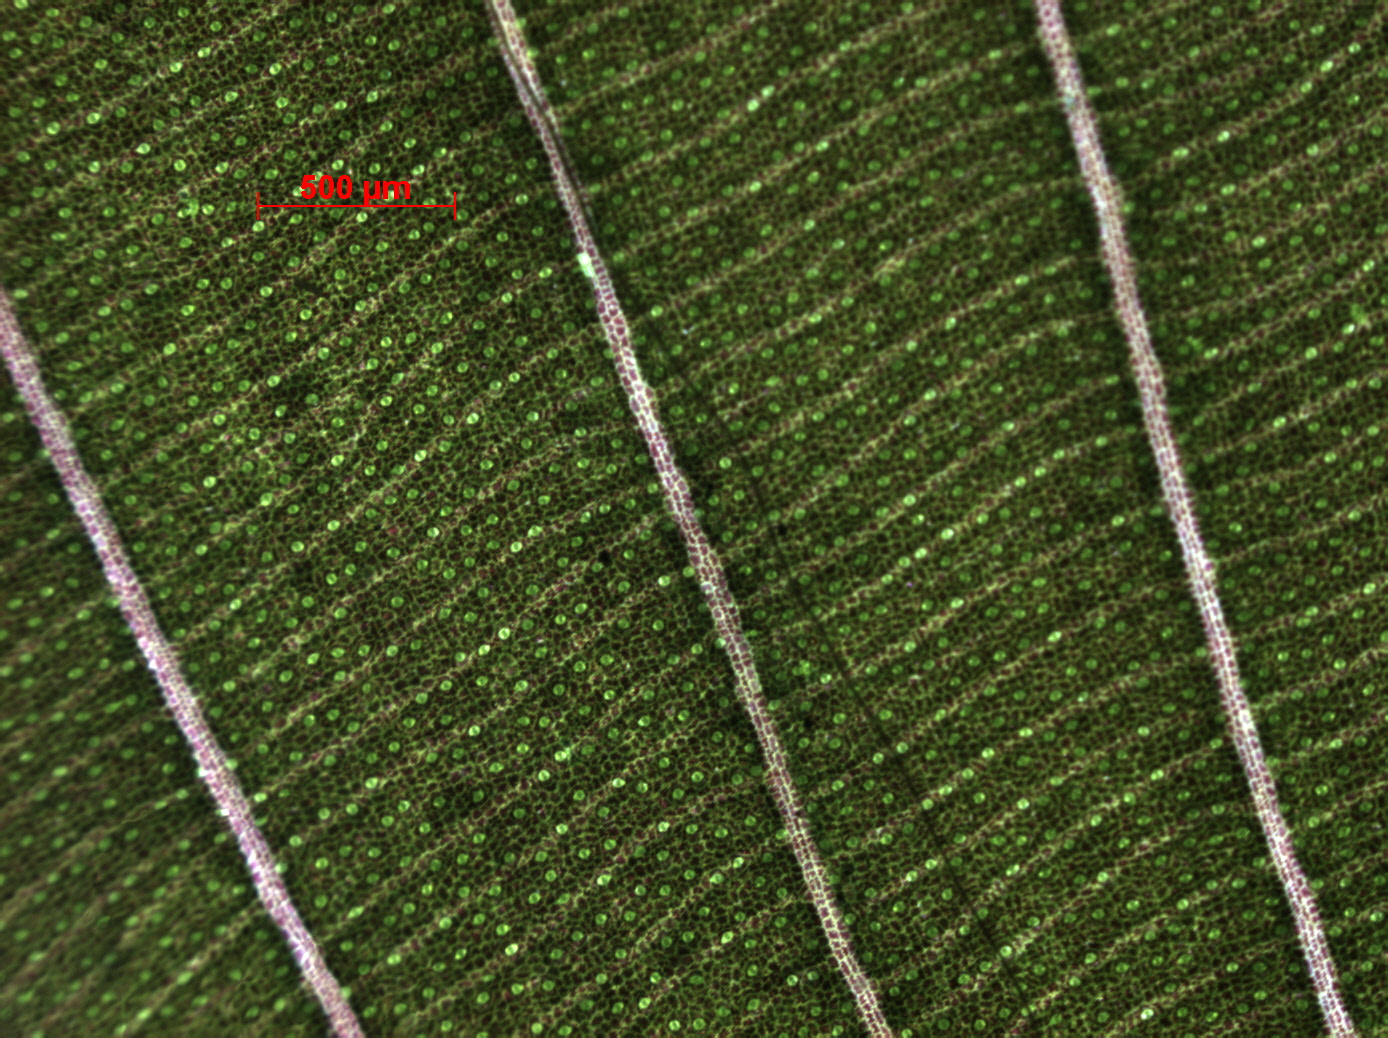
\includegraphics[scale=0.3]
			{images/fig1.png}
	\end{center}
	\centering
	\fautor
\end{figure}

There are several proposed methods to solve the sharpness problem in microscopy images, mostly based on image restoration techniques. According to \citeonline{ponti2016image}, the most frequently used iterative method in microscopic image restoration is the Richardson-Lucy algorithm. This is a particular case of the Maximum Likelihood Expectation Maximization algorithm with spectral extrapolation properties, which assists in the execution process at low conditions of \sigla{SNR}{Signal-to-Noise-Ratio}. Some examples presented by \cite{sun2005autofocusing} consist of
four classes: \emph{derivative algorithms}, \emph{statistical algorithms}, \emph{histogram-based algorithms} and \emph{intuitive algorithms}. Among these applications, derivative methods deserve more credit. The Fourier Transform proved itself to be
effective for low or moderate noise levels; in highly noisy environments, the resulting images were not satisfactory \cite{richardson1972bayesian}. From this evidence, probabilistic methods based on the Bayes Theorem were developed and provided images with better contrast, higher bandwidth and
edge enhancement for confocal fluorescence microscopy samples \cite{ponti2016image}.

The resulting images from such restoration processes have a higher degree of sharpness than the original ones when validated with metrics such as the \sigla{RMSE}{Root Mean Squared Error} and the \sigla{PSNR}{Peak Signal-to-Noise-Ratio} (both will be discussed further). However, the algorithms contain limitations when it comes to degradation as input; consequently, it produces degradation as output. An alternative to restoration is to use images from the same object, with different foci, in order to obtain an enhanced depth of field image with low degradation levels.

\section{Objectives and Hyphothesis}

The objective of this work is to develop a method which is capable of generating an extended depth of field image from a set of light microscopy images, acquired with different foci. The method will employ blur segmentation techniques and image fusion. The specific objectives are described as follows:

\begin{itemize}
    \item \emph{Evaluation of Blur Segmentation Methods}: Several approaches will be described to find the blur map, which employ different segmentation techniques. The aim is to find the approach that has the best behavior with multifocal light microscopy images. Based on current state-of-the-art literature, empirical results of efficiency and efficacy of the methods will be pursued, and a specific method for light microscopy will be developed. The performance evaluation relates to execution time, asymptotic complexity and blur map accuracy;
    
    
\end{itemize}

It is hypothesized that methods based on the Fourier and Wavelet Transforms may be employed to produce a reliable blur segmentation, in order to perform the multifocus image fusion and obtain an extended depth of field image.

\section{Structure of the document}

This monograph is organized as follows:

\begin{itemize}
    \item Chapter \ref{chapter:fundamentals-of-optics-and-light-microscopy} provides several essential concepts of Optics for understanding the Light Microscopy basics and the nature of blur;
    
    \item Chapter \ref{chapter:image-processing} contains the theoretical background in image processing, necessary for the comprehension of the related work and the proposed methods;
    
    \item Chapter \ref{chapter:related-work} apply the image processing basis and some other concepts with the most related relevant work in blur segmentation and multifocus image fusion areas;
    
    \item Chapter
    \ref{chapter:materials-and-methods} exposes details of the proposed approaches for solving the problem;
    
    \item Chapter \ref{chapter:preliminary-results}
    show some experimental results with artificially blurred images and real microscopy multifocus images;
    
    \item Chapter \ref{chapter:conclusions} is designed in this period for presenting the schedule of what should be done next in order to achieve the objective and use this work to contribute to science.
    
\end{itemize}


\chapter{Fundamentals of Optics and Light Microscopy}
\label{chapter:fundamentals-of-optics-and-light-microscopy}
Microscopes are instruments designed to accomplish several important tasks to human knowledge, either in the theoretical or the empirical domains. They are capable of magnifying images of small objects and structures, which could not be seen with ease by the human eye; this grants more information about the object of study to the research or the analysis. The first idea of the device was introduced by Romans, which discovered the magnifying property of glass in some sort of biconvex shape; furthermore, Robert Hooke and Anton van Leeuwenhoek (around 1665 and 1674, respectively) were the most prominent science-related men responsible for microscope improvements \cite{wu2008microscope}.

One of the important facts in science is the continuous technological improvement, which reflects on every field of study. Due to the development of theories and their empirical proofs of veracity, in addition to the advances in hardware and software power, techniques such as image processing are relentlessly applied into other fields. This also happens in microscopy, aiming to improve image quality, data reliability and range of use \cite{boyde1990modern}.

This chapter provides important information about light microscopy and optics, with regards to the project's scope. The first part is dedicated to the basic set of concepts and properties from optics that are necessary for light microscopy; the second one describes the structure of the optical microscope, along with its uses and implications on the acquired images. Plenty of image degradation causes lie on the system acquisition process; in fact, defocus is a natural occurrence in optics, mainly caused by adjustments of the optical system.

\section{Relevant elements of optics}

The definition of the spectroscopy procedure consists of the interaction between electromagnetic radiation and the matter \cite{gauglitz2006handbook}. This concept can be extended to microscopy, which deals with the section of the electromagnetic spectrum of wavelength comprehended between 400 and 700 nanometers, i.e. visible light,  to create visual representations of the objects
\cite{bell2009introduction}. Light microscopy is inherently related to optics, and some concepts of the field are directly related to the blurring process; therefore, it is meaningfully important to elucidate them.

\subsection{Dual Nature of Light}

Light was described in different ways according to different geniuses. Newton proposed that light had a corpuscular nature, due to the trajectory in which light appeared to travel in an uniform medium in his experiments; Huygens (1629 - 1695) affirmed in his works that light was traveling in a "wave-like" way and apparently could explain some optical principles such as the interference phenomena \cite{fowles1989introduction}.

Those were theoretical bases to the posterior studies of Maxwell, Planck, Einstein and Bohr \cite{fowles1989introduction}; these were responsible for linking the prior discoveries with the quantum theory, and therefore differ from this research's scope. Maxwell enunciated that there were two different vectors which could cause a state of disturbance in the space, while dealing with electric charges; those consist of the electric vector $\mathit{\mathbf{E}}$ and the magnetic induction vector $\mathit{\mathbf{H}}$, that together construct together the electromagnetic field \cite{born1999principles}, as shown in Figure \ref{fig:electromagnetic_wave}. 

\begin{figure}[htb]
	\centering
	\caption{\label{fig:electromagnetic_wave} 
		Composition of the electromagnetic wave. The red and the blue curves represent the electric and induction vectorial quantities, respectively.}
	\begin{center}
	    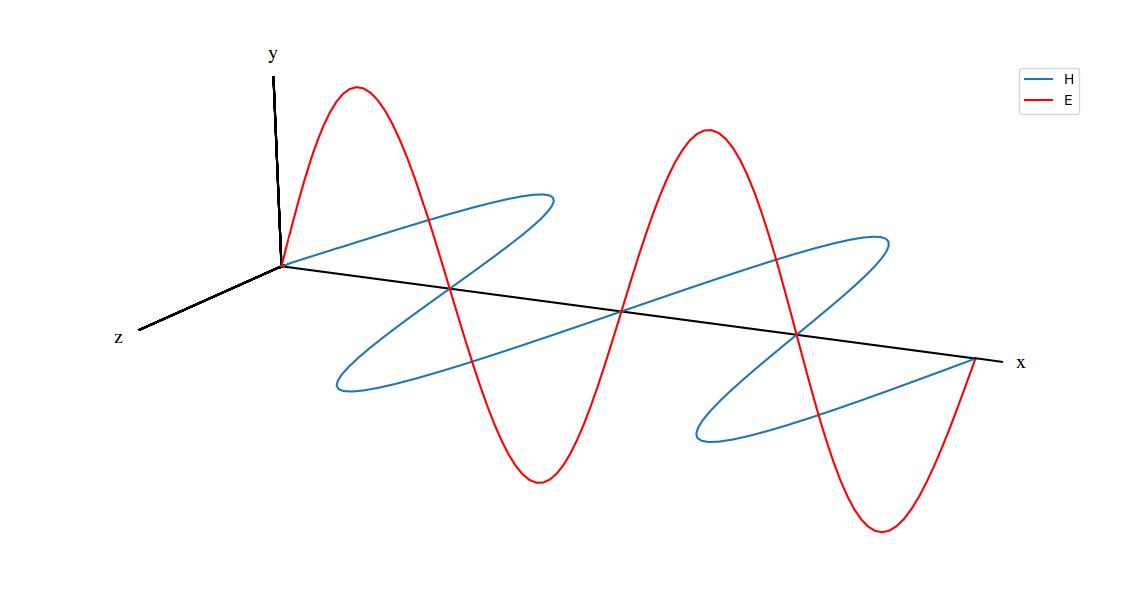
\includegraphics[scale=0.3]
			{images/fig2.png}
	\end{center}
	\centering
	\fautor
\end{figure}

Light as an electromagnetic wave is therefore composed by the two vectors and propagates in some particular coordinate direction upon a metric space, e.g. the $\mathit{x}$ coordinate on a three-dimensional euclidean space (Figure \ref{fig:electromagnetic_wave}). Hence, it is possible to treat light as a wave or particle, according to the application and its needs. Light microscopy deals with the wave model and its related phenomena such as reflection, refraction and diffraction, which will be presented on the posterior subsections and are useful for a deep understanding of the main object of this work: the blur effect.

\subsection{Light Wave Properties}

The light waves can be represented by a ray, i.e. a single oriented line which shows the direction of propagation; several waves that propagate in nearly the same direction can be named as a beam \cite{halliday2013fundamentals}. These two models of the real light are important and useful representations within the boundaries of visible light, and allow easier explanations of light properties.

A ray or a beam travels from a source, which may belong to picometric scales (due to nuclear processes) or to relatively higher scales, e.g. the fluorescent and incandescent light bulbs, which are sources of electric light. Eventually, light reaches surfaces during its propagation, and this is the event that allows the human vision feature; when it occurs, there are three prominent phenomena to consider: reflection, refraction and diffraction.

The incident ray of light suffers a split procedure when it reaches a frontier between two homogeneous media. One of the resulting rays proceeds the propagation process in the initial medium and the other one propagates inside the other medium; the first phenomenon is denominated \emph{reflection} and the second, \emph{refraction} \cite{born1999principles}. According to \citeonline{halliday2013fundamentals}, the reflection law states that the resulting ray lays within the incidence plane, and that the angle of reflection $\mathit{\theta^{'}_{1}}$ equals the $\mathit{\theta_{1}}$ angle of incidence; comparably, the refraction law states the same about the incidence plane and relates $\mathit{\theta_{1}}$ and $\mathit{\theta_{2}}$ angles by Snell's law, denoted by equation \ref{eqn:snells_law}. 

\begin{equation}
    \label{eqn:snells_law}
       n_{2}\sin{\theta_{2}} = n_{1}\sin{\theta_{1}}
\end{equation}

\noindent where $\mathit{n_{1}}$ and $\mathit{n_{2}}$ are the refractive indices of the media and represent the ratio of the speed of light in vacuum $\mathit{c}$ to the speed of light $\mathit{v}$ in the medium.
This framework consists in an approximation and may be considered ideal for didactic purposes. The process that happens in the real situations may involve non-homogeneous media, opaque or translucent media (which blocks the light propagation or change the direction of the rays randomly, respectively), and those concepts are relevant to the imaging procedures, e.g. microscopy. Figure \ref{fig:beam_split} depicts the real-world phenomenon and its ideal representation.

\begin{figure}[htb]
	\centering
	\caption{\label{fig:beam_split} 
	    (a) A beam of light falling onto a frontier between air and water, and suferring reflection and refraction. (b) Representation of the process in terms of rays.}
	\begin{center}
	    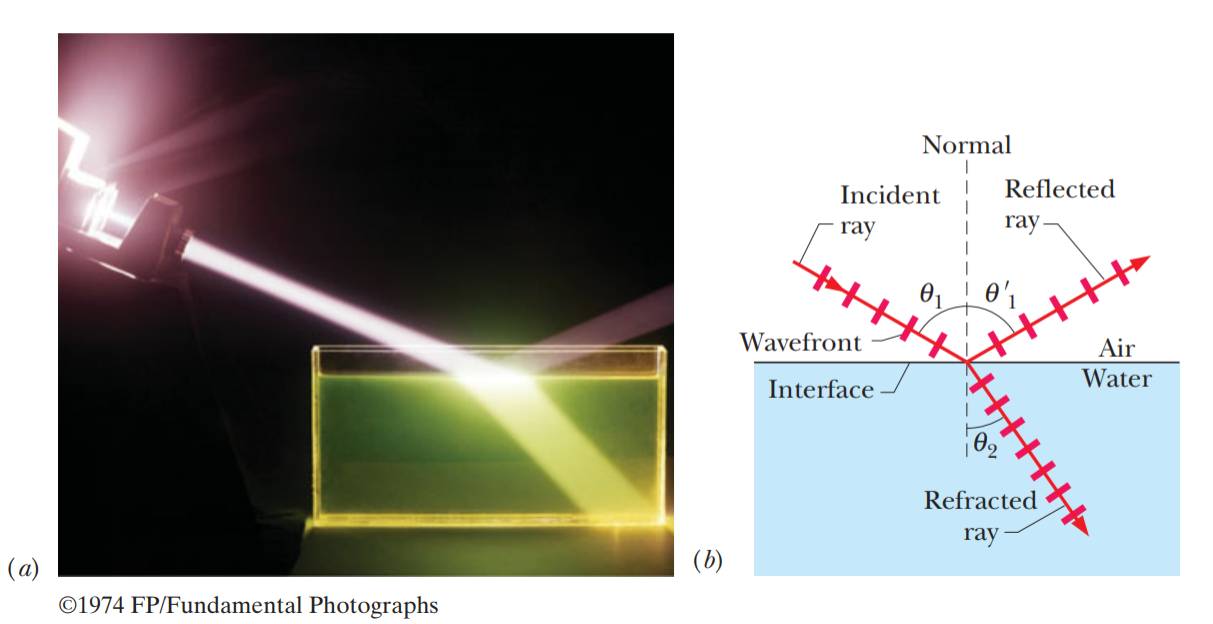
\includegraphics[scale=0.3]{images/fig3.png}
	\end{center}
	\centering
    \fdireta{halliday2013fundamentals}
\end{figure}

The wave theory of light also contains another important property for the real processes: the \emph{diffraction}. It consists of several occurrences that do not properly obey the geometrical optics patterns. When a beam of light reaches an opaque object, the waves suffer changes in their direction of propagation, which can be predicted by the fact that all the points in each wave front (points of identical phase on waves) generate a new wave, as stated by Huygens \cite{fowles1989introduction}. Therefore, the propagation of light in real-world situations involves some natural procedures that may influence the image formation and the image acquisition, by sensors or even by human beings.

\subsection{Imaging Properties of Optical Systems}

Within the scope of this work, the main reason for introducing the concepts of optics are the imaging devices - the microscope, in particular. The structure of the apparatus will be described in Section \ref{sec:light_microscopy}. Moreover, a substantially large amount of devices rely on optical lenses for imaging, with properties such as depth of field and depth of focus.

As stated by \citeonline{halliday2013fundamentals}, \emph{lenses} are objects consisting of a transparent material, with a certain refractive index, that are made of two spherical surfaces on which light propagates and suffers refraction. They are used in optical systems due to their capacity to create images as long as their refractive index is not equal to that of the medium. Still in agreement with \citeonline{halliday2013fundamentals}, some concepts related to lenses are important in our context and will be shown below. Figure \ref{fig:spherical_lens} denotes an illustration of an arbitrary spherical lens, and the following list depicts the principal elements from geometric optics that relates to lenses and its consequent imaging properties:

\begin{itemize}
    \item \emph{Radius of Curvature}: the distance between the center of the sphere and a refracting surface, named $\mathit{r_{1}}$ and $\mathit{r_{2}}$ on Figure \ref{fig:spherical_lens};
    
    \item \emph{Center of Curvature}: considering the fact that the lenses are made by an union of two sections of an sphere-shaped object (which have a center), there are two Centers of Curvature for each lens, denoted by $\mathit{C_{1}}$ and $\mathit{C_{2}}$ on Figure \ref{fig:spherical_lens};
    
    \item \emph{Central Axis}: a line that represents of the infinite number of radii of the sphere, which contain the center and the focal point;
    
    \item \emph{Focal Point}: also called \emph{focus}, a point within the central axis, where the image of the object is formed due to the convergence of the light rays from the object, and shown on Figure \ref{fig:spherical_lens} as $\mathit{F_{1}}$ and $\mathit{F_{2}}$;
    
    \item \emph{Focal Length}: presented as $\mathit{f}$ on Figure \ref{fig:spherical_lens}, it stands for the distance between the center of the sphere and the focal point;
    
    \item \emph{Object}: either a point or a surface on space that emits (or reflects) light and can be interpreted as a source;
    
    \item \emph{Image}: in this context, it is a representation of an object, formed by the action of lenses.
    
    \item \emph{Magnification}: a number that describes how larger or smaller the image will be in comparison to the object; mathematically, the ratio of the image distance to the object distance, both relative to the lens.
    
\end{itemize}

\begin{figure}[htb]
	\centering
	\caption{\label{fig:spherical_lens}Arbitrary scheme of the optical properties of a spherical lens.}
	\begin{center}
	    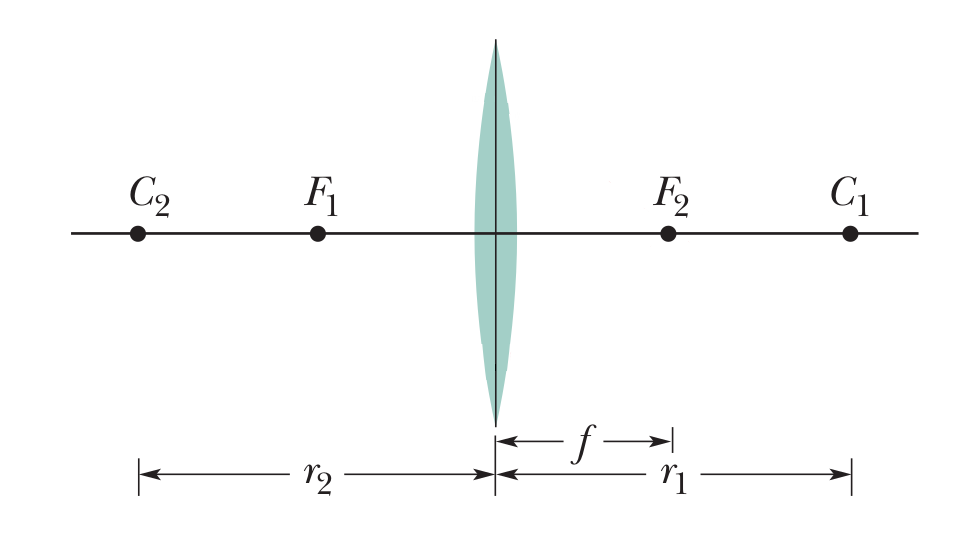
\includegraphics[scale=0.4]{images/fig4.png}
	\end{center}
	\centering
    \fadaptada{halliday2013fundamentals}
\end{figure}

A single lens or a set of lenses (most of the optical systems are more complicated than a single lens) have the \emph{depth of field} and the \emph{depth of focus} properties. Although the terms appear to be similar, the former relates to objects and the latter, to images \cite{davidson2002optical}. For every system, there is a focal plane in which the formed images will be sharp. Depth of Field is the tolerance for the object focal plane that may produce sharp images, whilst Depth of Focus dictates the same tolerance for the image focal plane. In other words, depth of field is the zone in the real world where focus will be acceptable and depth of focus is the same idea, for the imaging sensors or for plotting the image.

% %%%%%%%%%%%%%%%%%%%%%%% TO THE END
% Usually, objects in the real world do not have smooth surfaces.

% \cite{joshi2014defocus}

% the point spread function of an optical system and defocus.


\section{Light microscopy}
\label{sec:light_microscopy}

The type of microscope discussed and used in this work is the light microscope; there are several techniques and approaches for employing optical lenses in order to obtain magnified images, but they are outside the bounds of this research. The compound light microscope is a device designed to generate magnified images from objects with the aid of visible light, and consists of two lenses: the \emph{objective} (closer to the object) and the \emph{ocular} (closer to the observer) \cite{murphy2012fundamentals}. This section presents some concepts and principles from the field.

\subsection{General Structure}

As reported by \citeonline{bell2009introduction}, the basic structure of a microscope consists of objective lenses, eyepieces, condensers, the stage and the light source, which are graphically described by Figure \ref{fig:compound_microscope} and explained as follows:

\begin{itemize}
    \item \emph{Objective Lenses}: a set of multiple lenses merged inside a tubular structure (barrel), which are designed for capturing light rays from the specimen or object and are built for minimizing the series of optical unwanted phenomena in imaging;

    \item \emph{Eyepieces}: lenses where the observer may look through, also inside a tubular structure, but with lower magnification in comparison to the objective;
    
    \item \emph{Condensers}: a collector of light from the light source, which sends the focus the rays on the object;
    
    \item \emph{Stage}: the support for the object; which may have height and positional adjustments in some devices;
    
    \item \emph{Light Source}: the main source of light, usually a lamp.
\end{itemize}

\begin{figure}[H]
	\centering
	\caption{\label{fig:compound_microscope}Graphic representation of the basic compound light microscope structure.}
	\begin{center}
	    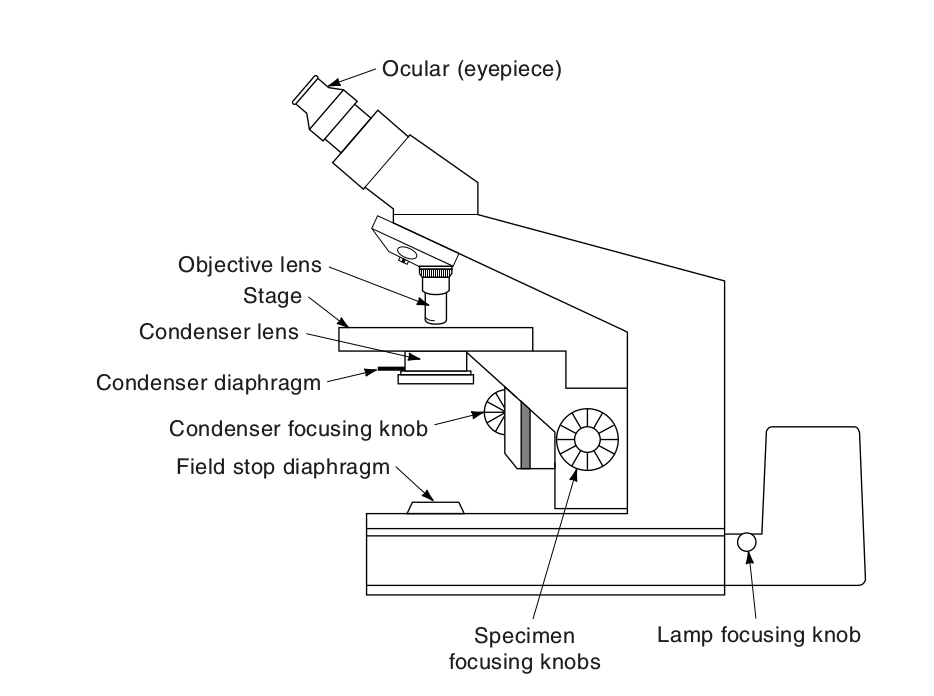
\includegraphics[scale=0.4]{images/fig5.png}
	\end{center}
	\centering
    \fdireta{bell2009introduction}
\end{figure}

Considering the fact that light is some sort of radiation, there are several different ways to achieve imaging in microscopes; it can be made by light, polarized light, lasers, X-rays, among others. There are also advanced techniques such as confocal microscopy, which is capable of imaging a very small area of the object, with all the light rays focused on it \cite{rochow1994introduction}. It all depends on the purpose of microscopy within the proposed task.

\subsection{Stereo Compound Microscope}


One of the versions of compound microscopes is the stereo microscope. It consists of a fusion of two compound microscopes in a convergent optical system, and may have two different objectives and eyepieces or only one objective and two eyepieces \cite{schreier2004advances}. The former is named \emph{binobjective-binocular} (Greenough) and the latter is named \emph{monobjective-binocular}, also named \sigla{CMO}{Common Main Objective Stereo Microscope}; the advantages of this type of microscope is the higher depth of field, that promotes ease of examination of biological specimens, relatively small materials and any kind of non-smooth surfaces, besides the view and acquisition of images on three dimensions \cite{rochow1994introduction}. The structure of both types of stereo compound microscopes are denoted by Figure \ref{fig:stereo_compound_microscope}

\begin{figure}[H]
	\centering
	\caption{\label{fig:stereo_compound_microscope}Graphic representation of the basic stereo compound light microscope structure, (a) for the Greenough type and (b) for the CMO.}
	\begin{center}
	    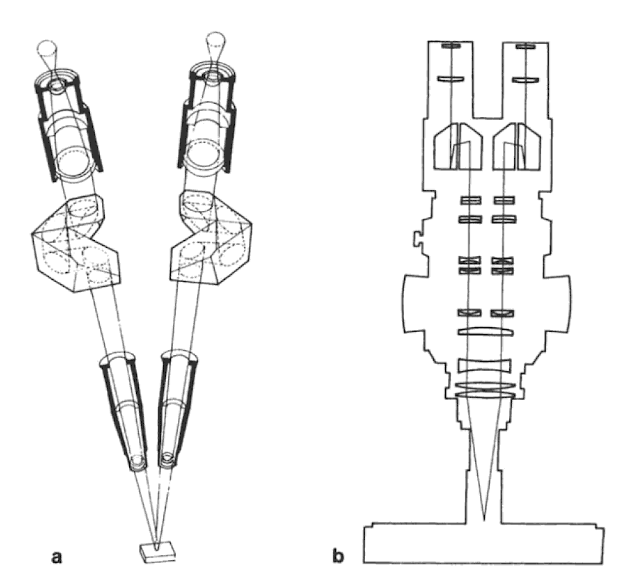
\includegraphics[scale=0.4]{images/fig6.png}
	\end{center}
	\centering
    \fdireta{rochow1994introduction}
\end{figure}

\chapter{Image Processing Techniques for Extended Depth of Field}
\label{chapter:image-processing}
%%%%%%%% symbols to add
\simbolo{\eta}{Additive noise function}
\simbolo{\ast}{Convolution operation}
\simbolo{\delta}{Dirac delta function}
\simbolo{\mathbb{R}}{Set of real numbers}
\simbolo{\mathbb{N}}{Set of natural numbers}
\simbolo{\wedge}{Diagonal matrix of decrescent multiple singular values}
\simbolo{\mathbb{G} = (\mathbb{V},\mathbb{E})}{Graph}
\simbolo{\mathbb{V}}{Set of vertices of a graph}
\simbolo{\mathbb{E}}{Set of edges of a graph}


This chapter aims to provide the necessary image processing background for the blur map construction and the image fusion procedure, as proposed by in the project. The approach for obtaining the blur map is an extension of the segmentation techniques, as they are created and used for extracting regions of interest in images. On the other hand, image fusion comprises a series of methods commonly applied in photography that will be addressed from a scientific point of view. Blur may have different causes such as movement, defocus, aberrations in the optical system, among others. All of them are addressed by researchers with image processing. On the other hand, image fusion can be seen as a decision problem, which can be dealt with a large amount of methods.

\section{Blur properties}

According to \citeonline{smith2007modern}, every optical system exhibits blur properties, in higher or lower proportions, due to the depth of focus and its adjustment. The defocus blur is caused by the incidence of light within an aperture with significant dimensions, where the source of light is not properly placed in accordance to the focal plane; it is related to the variables of the optical system such as depth of focus, aperture, depth of field, aberrations and so on \cite{joshi2014defocus}. Motion blur is caused by the attempt of taking pictures from moving objects and camera displacements; it can be caused in large scales (an image of a moving runner) or in small scales (live cell imaging). Both types of blur result in a loss of image details, sharpness and information. It can also be classified into global and partial blur. The former consists of a mathematically well-behaved homogeneous process and the latter is related to real world blurring phenomena. In light microscopy applications, the most relevant type is the partial defocus blur. Figure \ref{fig:defocus_motion_blur} shows an example of large scale defocus and motion blurs.

\begin{figure}[H]
	\centering
	\caption{\label{fig:defocus_motion_blur}Defocus blur (left) and motion blur (right) in large scales.}
	\begin{center}
	    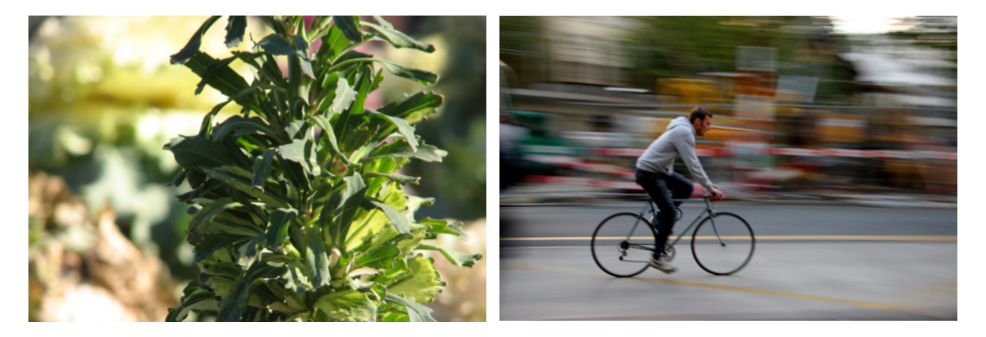
\includegraphics[scale=0.4]{images/fig7.png}
	\end{center}
	\centering
    \fadaptada{su2011blurred}
\end{figure}

\subsection{Point Spread Function}

Dirac delta functions are generalized functions designed for representing an impulse - a infinitely high value within a infinitely small period of time \cite{bracewell2000fourier}. In a nutshell, it is a function $\delta(x)$ that is zero-valued for any $x \neq 0$ and is infinity-valued for $x = 0$. This property can be combined with any smooth function $f\colon \mathbb{R}^{n} \to \mathbb{R}^{n}$, given  and provides the property shown in equation \ref{eqn:dirac_delta_function} in low dimension for didactic purposes. Figure \ref{fig:discrete_dirac_delta} illustrates the delta function on  $A = \{\, x\in \mathbb{R} \mid 0\le x\le 10^{7} \,\}$ normalized into the $[0,1]$ interval.

\begin{equation}
    \label{eqn:dirac_delta_function}
      \int^{\infty}_{-\infty}\delta(x-a)f(x) = f(a)
\end{equation}

\begin{figure}[H]
	\centering
	\caption{\label{fig:discrete_dirac_delta}Discrete representation of the Dirac delta function.}
	\begin{center}
	    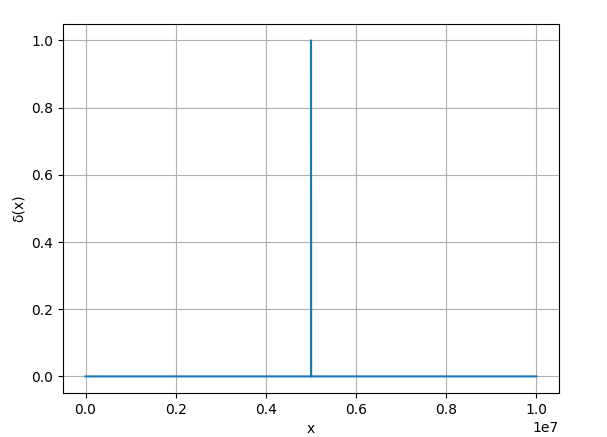
\includegraphics[scale=0.5, trim = {0 0.6cm 0 1.5cm}]{images/fig9.png}
	\end{center}
	\centering
    \fautor
\end{figure}

This concept of impulse is a light source with the shape of a point when it comes to images. It provides the effect of blurring on images, since it promotes the diffusion of the acquired information. Figure \ref{fig:psf} shows an arbitrary example of a punctual source of light and its image, which suffers the spreading effect.

\begin{figure}[H]
	\centering
	\caption{\label{fig:psf}Magnified image of a light impulse (left) and its impulse response function, the PSF (right).}
	\begin{center}
	    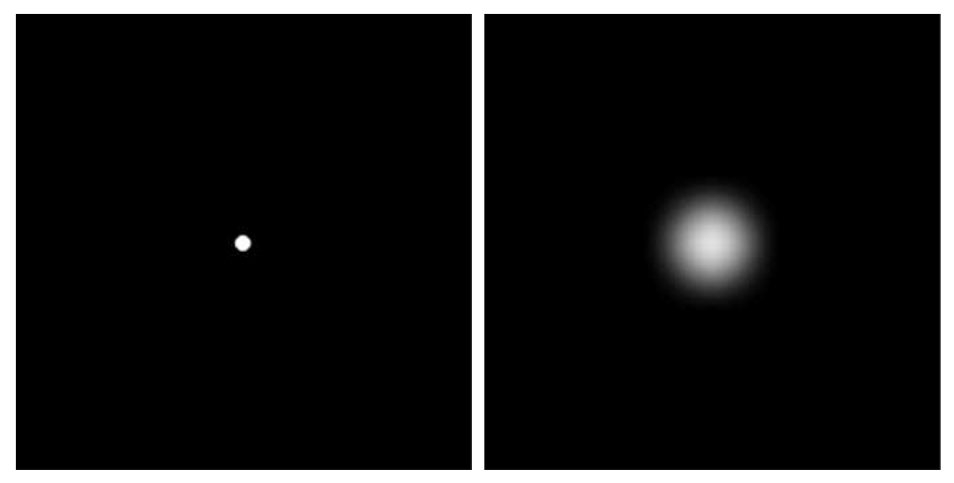
\includegraphics[scale=0.4]{images/fig8.png}
	\end{center}
	\centering
    \fadaptada{gonzalez2008digital}
\end{figure}

Digital images can be considered as discrete representations of a continuous space, as the image acquisition consists in the action of several sensors that capture light from the environment and divide the information into pixels. Hence, the most trivial and used representation for digital images are matrices of pixels and can be described as functions that suffer the influence of other functions during acquisition. The degradation process which stands for the influence quoted before may be mathematically illustrated by equation \ref{eqn:degradation_model} \cite{gonzalez2008digital}:

\begin{equation}
    \label{eqn:degradation_model}
       g(x,y) = h(x,y) \ast f(x,y) + \eta(x,y)
\end{equation}

\noindent where $f(x,y)$ is the function that represents the original image from the scene, $g(x,y)$ is the degraded image, $\eta(x,y)$ is the additive noise function and $h(x,y)$ is the point spread function of the imaging system. The $\ast$ symbol represents the convolution operation: in conformity with \citeonline{bracewell2000fourier}, it is an integral that relates a function $f$ with a function $g$ by means of a weighted sum in the range of a variable $u$, and is denoted by equation \ref{eqn:convolution}:

\begin{equation}
    \label{eqn:convolution}
       \int^{\infty}_{-\infty}f(u)g(x - u)du
\end{equation}

Thus, the blurring process can be considered as a natural phenomenon guided by a convolution operation, but it may suffer interference of factors such as motion of the object, the scene or the camera and differences of the surface's topology when it comes to microscopy. 

\section{Image Transforms}

Usually, the most trivial image processing operations are done at the pixel level; they act on one of the channels of an image from an specific color space, on gray levels of a grayscale image and so on. Some procedures such as the convolution have the computational performance as a bottleneck, and this is one of the reasons why \emph{image transforms} are widely used. They encompass any group of mathematical operations that takes the input signal or the input image out of their domain an project them onto the transformed domain \cite{gonzalez2008digital}. The convolution operation, for instance, turns itself into a simple matrix multiplication task on the Fourier Transform domain (which will be detailed in the following sections) and that solves the performance bottleneck. The general structure of a forward image transform and an inverse image transform is denoted by  the pair of equations \ref{eqn:generic_transform}, respectively:


\begin{align}
    \label{eqn:generic_transform}
    T(u,v) = 
    \sum_{x=0}^{M-1}
    \sum_{y=0}^{N-1}f(x,y)r(x,y,u,v)
    &&
    f(x,y) = 
    \sum_{x=0}^{M-1}
    \sum_{y=0}^{N-1}T(u,v)s(x,y,u,v)
\end{align}

\noindent where $M$ and $N$ are the dimensions of the image, $x$ and $y$ are coordinates of the image, $u = \{0,1,2,...,M-1\}$ and $v = \{0,1,2,...,N-1\}$ are called transform variables, $r(x,y,u,v)$ is a function named \emph{forward transform kernel} that is responsible for the forward domain change and finally $s(x,y,u,v)$ is the inverse kernel for $r$. These equations take an image to another domain, perform some operations and then return to the spatial domain. These are the common steps in transforms applications indeed. The following sections contain details about relevant image transforms in image segmentation and image fusion.

\subsection{Fourier Transform}

The Fourier Transform is a mathematical framework that expresses a periodic or non-periodic function with a sum of weighted sinusoids, what results in a set of different frequencies \cite{gonzalez2008digital}. The transform relies on complex numbers and the Euler's formula. The complex numbers belong to the broadest of the number sets, i.e. $\mathbb{R} \subseteq \mathbb{C}$, and consists of a \emph{real part} $a$ and an \emph{imaginary part} $bj$, shown by equation \ref{eqn:complex_number}:

\begin{equation}
\label{eqn:complex_number}
    z = a + bj
\end{equation}

\noindent where $j = \sqrt{-1}$ is the imaginary unit. In this sense, the Euler's formula relates complex exponential functions with trigonometric functions through the equation  \ref{eqn:euler_formula}:

\begin{equation}
\label{eqn:euler_formula}
    e^{j\theta} = \cos{\theta} + j\sin{\theta}
\end{equation}

\noindent where $\theta \in \mathbb{R}$ is a number that represents an angle in radians. This is the fundamental framework to describe the Fourier transform, since it is a sum of function representations by means of the Euler's formula. According to \citeonline{brigham1988fast}, the Continuous and the \sigla{DFT}{Discrete Fourier Transform} in a simplified version can be computed as shown on the left and on the right of Equation \ref{eqn:fourier_transform}, respectively:

\begin{align}
\label{eqn:fourier_transform}
    H(x) = \int_{-\infty}^{\infty}h(t)e^{-j2 \pi tx}dt
    &&
    H(x) = \sum_{x=0}^{N-1}h(t)e^{-j2 \pi t \frac{x}{N}}
\end{align}

\noindent with $H(x)$ as the Fourier transform of a function $h(t)$, $t$ represents functions is the time domain, $x$ represents the frequency domain and $N$ represents the total number of samples on the discrete approach. As already pointed out, images can be interpreted as two-dimensional functions; hence, the most important version of the Fourier transform in the context of image processing is the two-dimensional DFT, given by Equation \ref{eqn:2D_dft}:

\begin{equation}
\label{eqn:2D_dft}
    H(u,v) = \frac{1}{\sqrt{MN}}\sum_{x=0}^{M-1}\sum_{y=0}^{N-1}h(x,y)e^{-j2 \pi \big(\frac{ux}{M} + \frac{vy}{N}\big)}
\end{equation}

\noindent where $h(x,y)$ consists of an image, $M$ and $N$ are the image dimensions and $u$ and $v$ are coordinates in the frequency domain. This operation is extremely useful for almost every field related to analysis of functions. However, the DFT consists of a convolution process with $O(n^{2})$ asymptotic complexity, which can be too slow for larger dimensions. The \sigla{FFT}{Fast Fourier Transform} is an algorithm to compute the DFT by taking small slices of the signal, computing the transform with them and them merging the result. This procedure is performed in $O(n \log n)$ complexity, which is reasonable for many applications.

\subsection{Short-time Fourier Transform}

The set of advantages and applications of the FFT was already mentioned, but there is a remarkable property that should also be mentioned, since it has motivated the development of several other techniques: the FFT is a global transform. It transfers signals to the frequency domain, but does not take into account the local properties of the signal. The local histograms on an image may substantially vary, since it has different textures, edges, contrast, noise and even more features. The information about the position where a particular frequency occurs is also lost. Therefore, the solutions to the more complex analysis are the use of a \emph{Window Function} or the \emph{Multiscale analysis}.

The \sigla{STFT}{Short-time Fourier Transform} summarizes these concepts. It takes a particular window function, multiplies the signal with that window and performs the FFT, creating several output arrays representing each determined window size, i.e. sections of the signal. A window is a smooth function - a mask, in the discrete domain - which equals to zero on the boundaries of some interval. It is used to compute the STFT, hence it allows the local analysis of an image. One example of a discrete window function is the Hann window of length $L$ denoted by equation \ref{eqn:1D_hann}, as proposed by \citeonline{paukner2007foundations}:

\begin{align}
\label{eqn:1D_hann}
    w^{Hann}(x) - \frac{1}{2}
    \Bigg(
        1 - \cos\Bigg({\frac{2 \pi x}{L - 1}}\Bigg)
    \Bigg),
    &&
    x \in L
\end{align}

\noindent For two-dimensional windows, the tensor product of two windowing functions should be done. The STFT is therefore described by \citeonline{chikkerur2007fingerprint} equation \ref{eqn:2D_stft}:

\begin{equation}
\label{eqn:2D_stft}
    F(\tau_{1},\tau_{2},\omega_{1},\omega_{1}) = \int_{-\infty}^{\infty}\int_{-\infty}^{\infty}f(x,y)w(x-\tau_{1},y-\tau_{2}) e^{-j(\omega_{1}x + \omega_{2}y)}
\end{equation}

\noindent where $\tau_{1}$ and $\tau_{2}$ are spatial positions of the window and $\omega_{1}$ and $\omega_{2}$ are spatial frequency parameters.

\subsection{Wavelet Transform}

The Wavelet Transform is based on waves of varied frequency and limited time length, called "small waves" or wavelets \cite{gonzalez2008digital}.  Wavelets are functions that vary according to time or space and have oscillatory properties, such as a sine wave as defined by equation \ref{eqn:sinusoidal_wave}:

\begin{equation}
\label{eqn:sinusoidal_wave}    
    f(t) = A \sin{(\omega t + \varphi)}
\end{equation}

\noindent where $A$ is the wave amplitude, $\omega$ is the angular frequency and $\phi$ is the phase shift. The Fourier Transform also deals with this type of problem, and it is of utmost importance for mathematics, science and engineering
in general, in problems which are independent of time or consist of stationary states. Since Fourier Transforms can not carry information about time and frequency in parallel, wavelets are designed to help with those problems. Still according to \citeonline{gonzalez2008digital}, a wavelet transform may be seen as music sheet  that allows musicians to play certain notes at exact moments. 

The concepts of \citeonline{burrus1998introduction} will be used to clarify the mentioned transform. Wavelets are orthogonal functions (which means that their inner product equals to zero), represented by equation \ref{eqn:inner_product_wavelets}:

\begin{equation}
\label{eqn:inner_product_wavelets}    
    \langle \psi_{k}(t), \psi_{l}(t) \rangle = \int\psi_{k}(t)\psi_{l}(t)dt = 0
\end{equation}

\noindent where $\psi$ is a set of real-valued functions which can be substituted by any real-valued function $f$, which will lead to a coefficient instead of zero. The wavelet functions has a scaling function which originates the transforms, named \emph{mother wavelet} and represented by equation \ref{eqn:mother_wavelet}:

\begin{equation}
\label{eqn:mother_wavelet}    
    \psi_{j,k}(t) = 2^{j/2}\psi(2^{j}t - k)
\end{equation}

\noindent where $j,k \in \mathbb{Z}$ and $j$ is a scaling value. In this sense, the two-dimensional \sigla{DWT}{Discrete Wavelet Transform} is defined by equation \ref{eqn:dwt} \cite{gonzalez2008digital}:

\begin{equation}
\label{eqn:dwt}    
    W_{\psi}^{i}(j,m,n) = \frac{1}{\sqrt{MN}}\sum_{x=0}^{M-1}\sum_{y=0}^{N-1}f(x,y)\psi_{j,m,n}^{i}(x,y)
\end{equation}

\noindent where $W$ contains coefficients for horizontal, diagonal and vertical details for scales $j$. 

\section{Image Fusion}

Immediately upon the blur map extraction is satisfactorily complete, an image fusion operation is needed in order to achieve the highest amount of focused regions as possible. Image fusion is a process that merges several images (possibly taken in diverse conditions or with different cameras) into one image with higher quality, more details and consequently more useful for humans and computer tasks \cite{mitchell2010image}. Image fusion techniques can be used in noise reduction, edge enhancement and super-resolution, for example. 


%\textcolor{red}{paragrafo abaixo esquisito.. conversar..}

%Each image-related task defines what is relevant or not. The grayscale representation of \sigla{RGB}{Red, Green and Blue colourspace} may be enough either for human or computer evaluation; on the other hand, changes might be needed, e.g. noise reduction, edge enhancement and super-resolution. Combining several images is a technique to achieve those goals. 

One prominent use of image fusion occurs in medical image fields; the quality of information about illnesses, cells, clinical analysis and several other medical tasks (including the computer assisted ones) have found profitable results from the techniques and lead themselves to better and faster decisions when it comes to human beings \cite{james2014medical}.

There are relevant applications in remote sensing multispectral images, segmentation of regions in different colourspaces, biometry: the pan-sharpening process is the generation of an high resolution multispectral image from low to high resolution ones, K-Means segmentation and fusion of pixels in the \sigla{RGB}{Red, Green and Blue colourspace} and the Iris Recognition biometric process with video frames are examples of such tasks, respectively \cite{mitchell2010image}.

\subsection{General Framework}

Still according to \citeonline{mitchell2010image}, the general framework for the image fusion procedure can be accomplished in four stages: Multiple Input Images, Common Representational Format, Fusion and Display.
The \emph{multiple input images} stage consists in obtaining the set of images which will be merged. There are several approaches to this: the dataset may be captured from different sensors, on distinct light conditions or angles, with different magnifications, on several focus and with temporal measurements if the scene changes through time.

After the image set generation, there is the necessity of reshaping each item. This configures the \emph{common representational format}, responsible for creating a new and temporary dataset with the same properties, e.g. colourspace, dimensions, noise level and so on. The \emph{fusion} stage consists of using a decision method in order to dictate which regions, objects, colours or details will compose the final image; this can be done by any approach that relates to how the result should be. There are some methods that rely on the Wavelet Transform domain, for example. Finally, the \emph{display} stage consists in providing a view for the resulting image, which can be used directly for any further task or even be the input for other image processing operation. Figure \ref{fig:fusion_general_framework} depicts an arbitrary example of the four stages:

\begin{figure}[H]
	\centering
	\caption{\label{fig:fusion_general_framework}Image fusion general framework. (a) Multiple Input Images, (b) Common Representational Format, (c) Fusion and (d) Display.}
	\begin{center}
a 	    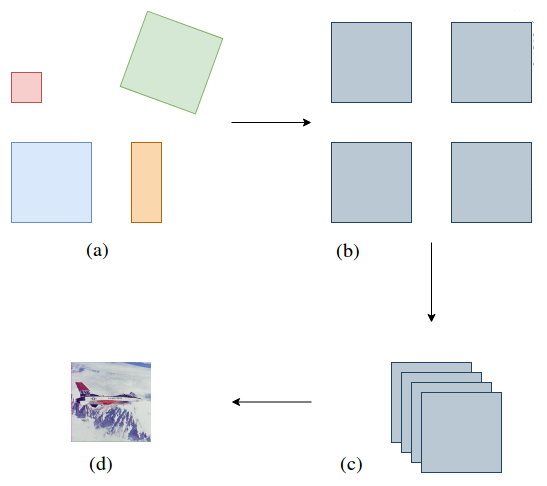
\includegraphics[scale=0.4]{images/fig10.png}
	\end{center}
	\centering
    \fautor
\end{figure}

The four arbitrary images in Figure \ref{fig:fusion_general_framework}.\textbf{(a)} represents different images of the same scene, taken at different resolutions, rotations and shapes. In \ref{fig:fusion_general_framework}.\textbf{(b)}, the images are all reshaped, converted to the same colourspace and ready to receive processing algorithm which will transform them into feature vectors. Figure \ref{fig:fusion_general_framework}.\textbf{(c)} represents the image fusion by means of an arbitrary method. The resulting image is depicted in Figure \ref{fig:fusion_general_framework}.\textbf{(d)}.

Since image fusion is only one branch of data fusion field, this procedure has a wide variety approaches and methods; hence, the domain will be restricted to the multifocus image fusion and some related work will be presented as follows, in section \ref{sec:multifocus_image_fusion}.


\chapter{Related Work}
\label{chapter:related-work}
The concepts presented in this chapter aims to introduce a review of the literature with relevant works on blur segmentation and multifocus image fusion. The methods in both fields are somehow related, as the output of a blurry region segmentation is the input for image fusion. The blur segmentation is mostly related to transform domain methods, but some of them also have simpler mathematical tools. In a nutshell, all of them are related to the standard image processing stages: pre-processing, particular operations, feature vector extraction and analysis. 

The literature review of multifocus image fusion shows that the trend is to use either more sophisticated methods or classic and well-known methods with enhancements in order to achieve the lossless image. Instead of just creating a blur map, the fusion works aim for a specific task which will presume that the image is at its best quality possible. 

\section{Blur Segmentation}

The main challenge of this project is to split the image between sharp parts and the blurred parts. The purpose of image segmentation techniques, according to \citeonline{petrou2010image}, is to extract regions that divide the image into sets of pixels with a common feature or characteristic. The extracted regions may be objects of interest for future processing or analysis. In our work, the objective is to obtain regions that were affected by the degradation process of blurring.

In agreement with \citeonline{uma2016comparison}, the segmentation of the unfocused regions of an image may be necessary for performing post-processing and restoration processes without affecting the sharp regions. This would allow feature extraction on these clear regions, which leads to a broad variety of analysis techniques. One of the principal elements of images that loses identity with the blurring process is the edge. Regardless of properties such as thickness, shape or irregularity, the edges consist of transitions that exhibit discontinuities of intensity. Edge detectors are mathematical operations capable of retrieving such discontinuities, which are identified as blur points and contrast differences \cite{barat2004segmentation}.

There are many techniques to obtain a map of blurry and sharp regions and many are based on solid mathematical concepts. In the next sections, the most relevant ones will be described: Haar Wavelets \cite{liang2017automatic}, Higher Order Statistics \cite{lee2014blurred}, Discrete Cosine Transform Coefficients \cite{taiebeh2017automatic} and Singular Value Decomposition \cite{su2011blurred}.

\subsection{Wavelet-based Segmentation}

\citeonline{liang2017automatic} proposed a Haar wavelet transform-based algorithm for blur detection and segmentation. The algorithm consists of blurring the image with a known blur kernel before performing the transform decomposition. This is due to the fact that there is a significant loss of detail after segmentation, which does not occur with such intensity if the image again undergoes a blurring process. This process can be done using a simple convolution by a Gaussian filter.

Next, the difference between the initial image and the convolved one is estimated. The result of this operation is the partially blurred image, and the third-order transform is applied
in blocks of 16x16 pixels around each pixel. Each block is decomposed into three sub-blocks of
$k = \{1, 2, 3\}$ order, denoted by $\{BH_k, BV_k, BD_k \}$, which stands for horizontal, vertical and diagonals, respectively. For all orders, the $L_p$ norm of each nine components of the block, as well as the attenuation ratio $a_k$ between the components of the same block in the image test and the convolved image. The amount of blur on any pixel $(i, j)$ is given by the product of the attenuation ratios of the three orders, as presented in equations \ref{eqn:blurriness} and \ref{eqn:blurriness_norm}:

\begin{equation}
\label{eqn:blurriness}
a_k(i,j) =
    \frac
        {
            \Big\{
                ||BH_k||_p + ||BV_k||_p + ||BD_k||_p
            \Big\}
            \Big|_{T_r}
        }
        {
            \Big\{
                ||BH_k||_p + ||BV_k||_p + ||BD_k||_p
            \Big\}
            \Big|_T
        }
\end{equation}

\begin{equation}
\label{eqn:blurriness_norm}
a(i,j) = \prod_{k=1}^3a_k(i,j)
\end{equation}

The resulting $a(i, j)$ value is normalized on the $[0,1]$ interval. The closer to 1, the greater the blurriness of the block on the test image; he closer to zero, the sharper the block.

\subsection{Higher Order Statistics-based Segmentation}

The statistical approach to blur segmentation proposed by \citeonline{lee2014blurred} consists
in extracting two features from the image: the \sigla{GM}{Gradient Magnitude} and the directional coherence. Higher Order Statistics based signal analysis is a tool for handling non-gaussian signals \cite{mitra2000nonlinear}. One of these techniques consists in computing the GM \cite{lee2014blurred}, that emphasizes the most intense discontinuity edges, suppresses the less intense ones and reduces noise. The framework to compute the GM is described by the equation \ref{eqn:GM} below.

\begin{equation}
\label{eqn:GM}
GM(i) = \log 
    \Bigg[
        \frac{1}{N_{P_i}}
            \sum_{j \in P_i} 
            \Bigg\{\sqrt{ \frac{I_x(j)^2 + I_y(j)^2}{2}} \Bigg\}^k
    \Bigg]
\end{equation}

\noindent where $I_x$ and $I_y$ are values that represent the intensity gradient in vertical and horizontal directions, respectively. $P$ represents the considered region in an iteration, centered on the $i-th$ pixel, and $N$ represents the number of pixels in $P$. The $k$ value indicates the statistical order.

\sigla{DC}{Directional Coherence} is a measure of local similarities of a scene. It can be computed, according to \citeonline{lee2014blurred}, by applying the \sigla{ST}{Structural Tensor}, which divides the dominant directions and the coherence's directions in the local region, as depicted by equation \ref{eqn:ST}:

\begin{equation}
\label{eqn:ST}
ST(i) =
    \begin{bmatrix}
        \sum_{j \in P_i}I_x(j)^2  & \sum_{j \in P_i}I_x(j) + I_y(j) \\
        \sum_{j \in P_i}I_x(j) + I_y(j) & \sum_{j \in P_i}I_y(j)^2 
    \end{bmatrix}
\end{equation}

\noindent ($I_x$, $I_y$, $P$ and $N$ are the same as described in Equation \ref{eqn:GM}). The eigenvalues of the ST tensor specify the degree of the anisotropy of the gradient distribution in $i-th$ region. Finally, equation \ref{eqn:DC} defines the directional coherence.

\begin{equation}
\label{eqn:DC}
DC(i) =
    \Bigg(
        \frac{\lambda_1 - \lambda_2}{\lambda_1 + \lambda_2}
    \Bigg)^2
\end{equation}

\noindent where $\lambda_{1}$ and $\lambda_{2}$ are the eigenvalues of the $ST$ matrix. After obtaining the feature vectors, it is possible to use a classifier - a function or a set of them, which labels the elements in distinct classes - and define whether each pixel is blurry or not. If prior information is provided to the classifier, it will characterize an example of supervised learning; otherwise, it will need to be able to
infer similarities within the sample from the feature vectors, consisting in an unsupervised learning procedure. The \sigla{SVM}{Support Vector Machine} classifier can be trained and applied to determine the blurry and sharp sets of pixels.

\subsection{Discrete Cosine Transform Coefficients Based Segmentation}

The procedure which \citeonline{taiebeh2017automatic} proposed also takes into account the fact that blurred regions, before and after a second similar degradation process, have small differences when compared; besides, the differences between the sharp regions on the same metric are relevant. This peculiarity can also be verified in the \sigla{DCT}{Discrete Cosine Transform} domain: most of the high frequency coefficients are lost and the difference quoted above may be used to estimate the amount of blur in the image. 

The DCT is an important mathematical operation, commonly used in data compression and signal processing, which takes sets of values and outputs transform coefficients; its two-dimensional version is executed in blocks (small sets of pixels) and is shown by equation \ref{eqn:dct} \cite{salomon2007data}:

\begin{equation}
    \label{eqn:dct}
    G_{ij} = \sqrt{\frac{2}{m}}
             \sqrt{\frac{2}{n}}
             C_{i} C_{j}
             \sum_{x=0}^{n-1}
             \sum_{y=0}^{m-1}
             p_{xy}
             \cos 
                \Bigg[
                \frac
                {(2y + 1)j\pi}
                {2m}
                \Bigg]
            \cos 
                \Bigg[
                \frac
                {(2x + 1)i\pi}
                {2n}
                \Bigg]
\end{equation}

\begin{align*}
C_{i} =
\begin{cases} 
    \frac{1}{\sqrt{2}} & \text{$i = 0$,} \\
    1 & \text{$i > 0$},
\end{cases}
&&
i\in \mathbb{N} \mid 0\leq i < n
&&
C_{j} =
\begin{cases} 
    \frac{1}{\sqrt{2}} & \text{$j = 0$,} \\
    1 & \text{$j > 0$},
\end{cases}
&&
j\in \mathbb{N} \mid 0\leq j < m
\end{align*}

\noindent where $p_{xy}$ is the matrix which represents the image, $m$ and $n$ are the image dimensions. As described in the equation \ref{eqn:lp_norm_ratio}, the blur metric $\beta$ consists of the quotient between the $L_p$ norm of the original blurred image coefficients and the ones from the reblurred image.

\begin{equation}
\label{eqn:dct_image}
	\mathbf{D} = DCT(\mathbf{I})
\end{equation}

\begin{equation}
\label{eqn:dct_reblurred_image}
	\mathbf{D}_b = DCT(\mathbf{I}_b)
\end{equation}

\begin{equation}
\label{eqn:lp_norm_ratio}
	\beta(\mathbf{I}) = \frac{||\mathbf{D}_b||_p}{||\mathbf{D}||_p}
\end{equation}

\noindent where $\mathbf{I} \in \mathbb{R}^{2}$ is the original image and $\mathbf{I}_b \in \mathbb{R}^{2}$ is the re-blurred image with a low-pass filter (mean filter), $\mathbf{D} \in \mathbb{R}^{2}$ and $\mathbf{D}_b \in \mathbb{R}^{2}$ are the discrete cosine transforms of $\mathbf{I}$ and $\mathbf{I}_b$, respectively. The $L_p$ norm is defined by the equation \ref{eqn:lp_norm}:

\begin{equation}
\label{eqn:lp_norm}
	||\mathbf{D}_b||_p = \sum_{u,v}{(|\mathbf{D}_b(u,v)|)^p}
\end{equation}

\noindent The $\beta$ value is normalized on the $[0,1]$ interval; the closer to 1, the greater the amount of blur. This measurement is applied pixel by pixel in blocks of experimentally determined sizes such as 45x45, 19x19 and 9x9. The final blur measure for each pixel is an average of the measurements of the three blocks, and provide a substantially accurate blur map.

The acquired blur map is smoothed between regions and allows to infer significant differences between the sharp and blurred ones. The segmentation process is based on the map, and uses the concept of \emph{pixon} (set of related pixels with similar properties as colour, intensity, texture, among others): the problem is based on classifying such sets of pixels. In order to create the pixel set, a blur map scan is performed in the neighbourhood of each pixel; the neighbours are joined to the pixons that have the average value closest to a certain threshold; otherwise a new pixon is created.

The pixon set extraction divides the blur map in a set of sub-regions which will be classified as blurred or sharp. The \sigla{FCM}{Fuzzy C-Means Algorithm} was used by \citeonline{taiebeh2017automatic} and consists of the following steps:

Let $M$ be the set of pixels with their respective intensities, $C$ be the number of classes (two, in this case) and $w\in \mathbb{R} \mid 1 < w < \infty$ be the fuzzy exponent.

\begin{enumerate}[label=\Roman*.]

    \item The fuzzy association functions $u_ {c, m}^{(0)}$ must be initialized with $c = {1,..., C}$ and $m = {1, ..., M}$, which are entries for an $\mathbf{U}^{(0)}$ array of $C$x$M$ dimensions;
    
    \item For each iteration $l = {1,2,3,...,L}$, the centroids ${v_ {c}}^{l}$ of each cluster are computed by means of the equation \ref{eqn:fuzzy_cluster_center}:
    
    \begin{equation}
    \label{eqn:fuzzy_cluster_center}
    	v_{c}^{l} = \frac{\sum_{m=1}^{M}(u_{c,m})^{w}x_m}{\sum_{m=1}^{M}(u_{c,m})^{w}}
    \end{equation}

    \item Update the $\mathbf{U}^{(l)}$ array through the equation \ref{eqn:update_matrix}:
    
    \begin{equation}
    \label{eqn:update_matrix}
    	u_{c,m} = \frac{1}{\sum_{i=1}^{C}\Big(\frac{d_{c,m}}{d_{i,m}}\Big)^{\frac{2}{w-1}}}
    \end{equation}
    
    \noindent where $d_{i,m}^2 = ||x_m - v_i||^2$ and $||.||$ stand for the Euclidean Norm.
    
    \item Compare $\mathbf{U}^{(l)}$ and $\mathbf{U}^{(l+1)}$. If $||\mathbf{U}^{(l)} - \mathbf{U}^{(l+1)}|| \leq \varepsilon$, the classification procedure halts; otherwise, it goes back to step II.

\end{enumerate}

\noindent The $w$ value determines the clustering imprecision; it has been empirically determined by the authors that $w = 2$ and $\varepsilon = 0.00005$ are appropriate choices.

\subsection{Singular Value Decomposition-based Segmentation}

\citeonline{su2011blurred} proposed a 
\sigla{SVD}{Singular Value Decomposition}-based blur segmentation approach. It is a Linear Algebra derived technique of great utility, in which an array can be represented by multiple matrices of rank 1 (in this case, they can be denominated \emph{eigenimages}). The matrix equation \ref{eqn:basic_svd}
illustrates the SVD procedure on an image.

\begin{equation}
\label{eqn:basic_svd}
	I = U{\wedge}V^{T}
\end{equation}

\noindent where $I$ is a matrix that represents the image, $U$ and $V$ are orthogonal arrays and $\wedge$ is a diagonal matrix, composed of multiple singular values sorted in descending order. The decomposition of the image can be represented more specifically by the equation \ref{eqn:svd}:

\begin{equation}
\label{eqn:svd}
	I = \sum_{i=1}^{n}\lambda_{i}{\mathbf{u}_i}{\mathbf{v}_i}^{T}
\end{equation}

\noindent where $\mathbf{u}_i$, $\mathbf{v}_i$ are column vectors of $U$ and $V$, and $\lambda_{i}$ are the diagonal terms of $\wedge$. This process decomposes the image into a weighted sum with a certain amount of eigenimages, where the weights are singular values. Image details are captured as if it was a compression procedure, in which only $k$ singular values are considered.

Eigenimages act as multiscale analysis tools: the first most significant eigenimages involve larger scales, which provide the coarser formats; similarly, the remaining products of the decomposition provide details. Considering the convolution of a PSF $H$ with the image $I$, the high frequencies that represent the details are lost, i.e. the small singular values will correspond to larger values after the process. A blurred image has the first most significant eigen with larger singular values. The authors in \citeonline{su2011blurred} proposed a metric quantify the degree of blurriness of the image is proposed by the equation \ref{eqn:svd_blur_metric}:

\begin{equation}
\label{eqn:svd_blur_metric}
	\beta_{1} = \frac{\sum_{i=1}^{k}\lambda_{i}}{\sum_{i=1}^{n}\lambda_{i}}
\end{equation}

\noindent where $\lambda_{i}$ is the computed singular value for the neighbourhood of a given pixel. The metric is capable of classifying all pixels of the image in blurry or sharp with a threshold-based comparison; the result of the process is also a blur map.


\section{Multifocus Image Fusion}
\label{sec:multifocus_image_fusion}

Either in microscopic or macroscopic scales, imaging devices have a finite depth of field. All the slices of the image which are blurry came from the fact that a subset of pixels might be acquired outside the boundaries of depth of field \cite{huang2007evaluation}. Therefore, it is nearly impossible to obtain a globally sharp image in microscopic scales, since the differences of heights within the surface of the sample will also be magnified and the depth of field of microscopes is usually small in those cases. Image fusion is what may provide a fully sharp image, if a stack of images is acquired with a variety of focus adjustments.

The most trivial pixel-level fusion techniques are simple mathematical operations such as the average or a weighted average of gray levels; those are capable of performing the task, but also deliver some losses in basic image features, e.g. contrast and saturation \cite{zhang2009multifocus}. Thus, there is a demand for techniques that rely on more sophisticated tools, capable of covering multiple situations: images taken in different resolutions, light conditions and exposure times, for instance. Multiscale transform approaches, e.g. wavelet domain transforms, are a good choice for the problem and provide a very flexible framework, since it depends on the chosen wavelet function \cite{pajares2004wavelet}.

Most of the methods work upon the transform domain space, but there are also some noteworthy ones which are based on different basis. The following sections will elucidate multifocus image fusion techniques such as Graph and Spatial Frequency \cite{li2008multifocus} and Wavelet Transform \cite{pajares2004wavelet}.
% and Principal Component Analysis \cite{naidu2008pixel}.

% Nonsubsampled Contourlet Transform \cite{zhang2009multifocus}

\subsection{Graph and Spatial Frequency-based Fusion}

\citeonline{li2008multifocus} proposed an approach for the multifocus image fusion task that works on the spatial domain and has two fusion stages: the image is fused with the simple average method, then a segmentation procedure is performed by means of graph algorithms; the result is a region split of the initial images, which will be fused again with a spatial frequency technique.

Let $\mathbb{G} = (\mathbb{V},\mathbb{E})$ be the representation of a undirected weighted graph, where $\mathbb{V} = \{v_{1},v_{2},...,v_{n}\}$ is the set of vertices that stands for the pixels of the image and $\mathbb{E} = \{e_{1},e_{2},...,e_{m}\}$ is the set of edges that connect each pair of nodes based on the similarity degree shown by $\mathbf{W}(i,j)$, the weight function. The Normalized Cut algorithm is responsible for dismembering the graph into two complementary sets $A$ and $B$, and its threshold value for cutting edges is defined by equation \ref{eqn:ncut_base}

\begin{equation}
\label{eqn:ncut_base}
    Ncut = 
    \frac{cut(A,B)}{assoc(A,\mathbb{V})} +
    \frac{cut(A,B)}{assoc(B,\mathbb{V})}
\end{equation}

\noindent where $cut(A,B)$ is the sum of 
weights from $A$ to $B$, $assoc(A,\mathbb{V})$ and $assoc(B,\mathbb{V})$ are the sums of weights from $A$ an $B$ to the whole graph, respectively.

Considering $T$ as a input image, $(i,j)$ as indices for nodes, $\mathbf{F}(i)$ as intensity value for node $i$, $\mathbf{X}(i)$ as the coordinates of node $i$ and $\sigma$ as a coefficient set within 10\% and 20\% of the distance range, the proposed segmentation algorithm is organized in the following steps, as shown by \cite{li2008multifocus}:
    
\begin{enumerate}[label=\Roman*.]
    \item Build the graph with the chosen distance or similarity function and build two matrices $\mathbf{W}$ and $\mathbf{D}$, where
    
    \begin{align*}
        \mathbf{W}(i,j) = 
        \exp{\frac{-||\mathbf{F}(i)-\mathbf{F}(j)||_{2}^{2}}{\sigma_{I}^{2}}} t,
        &&
        t = 
        \begin{cases}
            \exp{\frac{-||\mathbf{X}(i)-\mathbf{X}(j)||_{2}^{2}}{\sigma_{X}^{2}}} & \text{if}
            ||X(i)-X(j)||_{2} < r
            \\0 & \text{otherwise}
        \end{cases}
    \end{align*}
    
    where $r$ is a threshold to create zeroes in $\mathbf{W}$ if the nodes have a greater distance in comparison to it and $\mathbf{D}$ is the diagonal matrix of cumulative sums for each node;
    
    \item The next step consists in computing the eigenvectors of $(\mathbf{D} - \mathbf{W})\mathbf{x} = \lambda\mathbf{D}\mathbf{x}$ with the smallest eigenvalues and minimizing the $Ncut$ function in order to perform a partition on the graph;
    
    \item Finally, check the stability of the partition by comparing the ratio between minimum and maximum of the histogram of eigenvectors values to an empirically determined threshold, $0.06$.
\end{enumerate}

With the two graph representations of image regions in hands, it is now possible to apply the spatial frequency procedure to recast the image. The metric relies on two values $RF$ and $CF$ (row frequency and column frequency), computed by equations \ref{eqn:rf} and \ref{eqn:cf}:

\begin{equation}
\label{eqn:rf}
    RF = \sqrt{\frac{1}{MN}
    \sum_{M-1}^{m=0}
    \sum_{N-1}^{n=1}
    [\mathbf{F}(m,n) - \mathbf{F}(m,n-1)]^{2}}
\end{equation}

\begin{equation}
\label{eqn:cf}
    CF = \sqrt{\frac{1}{MN}
    \sum_{N-1}^{n=0}
    \sum_{M-1}^{m=1}
    [\mathbf{F}(m,n) - \mathbf{F}(m-1,n)]^{2}}
\end{equation}

\noindent where $M$ and $N$ are the dimensions of the image and $\mathbf{F}(m,n)$ is intensity value of pixel at the position $(m,n)$. The spatial frequency is obtained by equation \ref{eqn:cf}:

\begin{equation}
\label{eqn:sf}
    SF = \sqrt{(RF)^{2} + (CF)^{2}}
\end{equation}

The spatial frequency index is then computed for every region of $A$ and $B$ subgraphs, and a decision task occurs as mathematically described in equation \ref{eqn:rof}:

\begin{equation}
\label{eqn:rof}
    RoF_{i} = 
    \begin{cases}
        RoA_{i}, & SF_{i}^{A} \geq SF_{i}^{B}\\
        RoB_{i}, & SF_{i}^{A} < SF_{i}^{B}
    \end{cases}
\end{equation}

\noindent where $i$ denotes the $i$-th region that is being calculated and the SF indices stand for correspondent regions in $A$ and $B$. If there are other images on the initial set, the process occurs in iteration for each of them.

\subsection{Wavelet Transform-based Fusion}

The modus operandi proposed by \citeonline{pajares2004wavelet} with the employment of the wavelet transform is relatively simple. It consists of applying the two-dimensional DWT in order to decompose the image in four common frequency bands for wavelet transforms as show in Figure \ref{fig:filter_banks}, where $h_{0}$ is the high band, $h_{1}$ is the low band, $f(m,n)$ is the input image and $2\downarrow$ stands for the downsampling operator that reduces the input size by half. Subsequently, there are some heuristics to merge the DWT coefficients and consequently the images.

\begin{figure}[htb]
	\centering
	\caption{\label{fig:filter_banks}Two-dimensional filter bank with four frequency bands.}
	\begin{center}
	    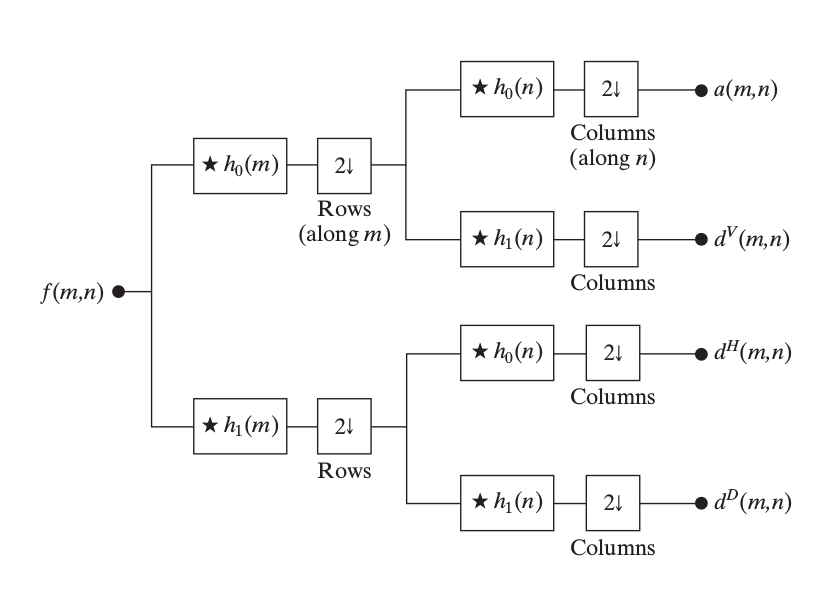
\includegraphics[scale=0.4]{images/fig11.png}
	\end{center}
	\centering
    \fdireta{gonzalez2008digital}
\end{figure}

Then, the coefficients will go through a thresholding procedure: the minimum value for taking a coefficient as significant may be obtained by the relationship of the standard deviation $\sigma$ of them all and the total size $n$ of the input: $T = \sigma\sqrt{2logn}/\sqrt{n}$. With the values from the last processing stage in hands, the fusion procedure happens with a \emph{fusion rule}, i.e. the heuristic to pick the right pixel value on each matrix in order to obtain the best fused image possible. All the values to be merged must represent the same resolution level, despite the decomposition level and the frequency band. For the multifocus image fusion, \citeonline{pajares2004wavelet} suggest the use of \sigla{CM}{Choose-Max} and \sigla{AWA}{Adaptive Weighted Average} heuristics. The CM depends on a property named activity level of the regions, represented by equation \ref{eqn:activity_level}

\begin{equation}
    \label{eqn:activity_level}
    A_{I}(p) = |D_{I}(p)|
\end{equation}

\noindent where $p = (m,n,k,l)$ is a tuple that represent a pixel in one of the decomposition levels: $m$ and $n$ indicate the spatial position in a given
frequency band, $k$ the decomposition level, and $l$ the frequency band. $D$ is a matrix with the coefficients from the decomposed image. To compute the elements that will compose the fused image, the CM procedure uses the maximum value of the same position in the two or more images, as shown by equation \ref{eqn:cm}

\begin{equation}
    \label{eqn:cm}
   CM = \max(A_{X}(p),A_{Y}(p))
\end{equation}

\noindent The AWA heuristic computes weights for each pixel with the expression in equation \ref{eqn:awa}:

\begin{equation}
    \label{eqn:awa}
   AWA = |D_{X}(p) - \Bar{D}_{X}(p)|^{a}
\end{equation}

\noindent with $\Bar{D}_{X}(p)$ representing the complementary set of positions to $D_{X}(p)$ and $a$ consisting of an exponent to modify the weight distribution. In order to finish the stack of operations and obtain the final fused image, it is only necessary to apply the \sigla{IDWT}{Inverse Discrete Wavelet Transform}.


\chapter{Materials and Methods}
\label{chapter:materials-and-methods}
The diagram on Figure \ref{fig:processing_flow} illustrates the proposed methodology to achieve the extended depth of field. The framework can be divided into four parts, as follows:

\begin{figure}[H]
	\centering
	\caption{\label{fig:processing_flow}Generic processing flow of the extended depth of field task: Image Acquisition \textbf{(I)}, Image Pre-processing \textbf{(II)}, Image Segmentation \textbf{(III)}, Image Fusion \textbf{(IV)} and Evaluation \textbf{(V)}.}
	\begin{center}
	    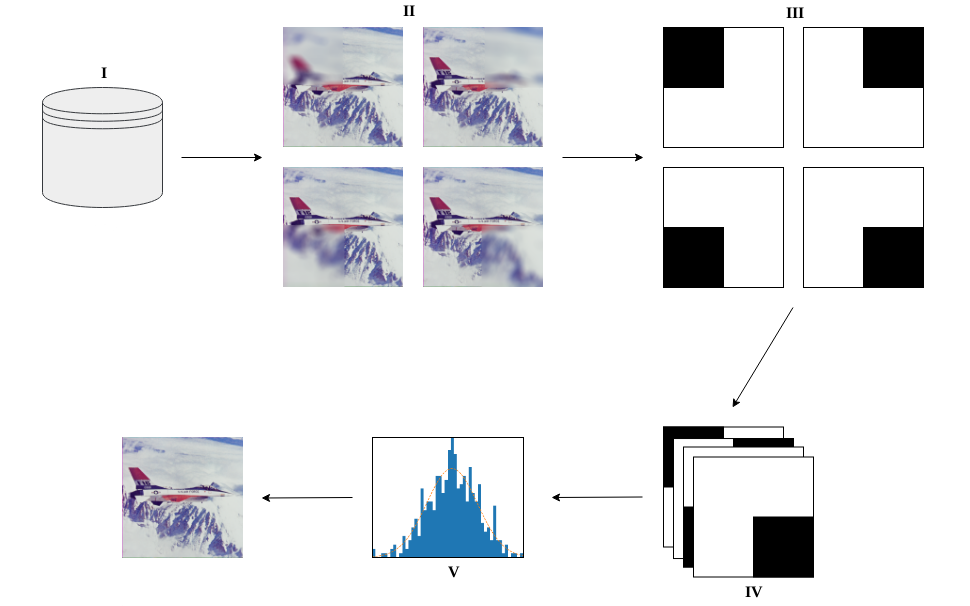
\includegraphics[scale=0.35, trim = {0 0.3cm 0 2cm}]{images/fig12.png}
	\end{center}
	\centering
    \fautor
\end{figure}

\begin{enumerate}[label=\Roman*.]
    \item \textbf{Image Acquisition}: several images will be acquired in different focus settings with the light microscope. The AxioVision 4.8 acquisition module tool called \emph{Z-Stack} allows to acquire images along the $z$ axis with a motorized focusing device that provides steps between each image with micrometer scale precision. This will result in a set of images with different levels of blur;
    
    \item \textbf{Image Pre-processing}: some adjustments are necessary prior to segmentation. The original image stack is in the RGB colour space. There was a conversion to colour spaces such as the \sigla{HSV}{Hue, Saturation and Value colour space}, in which the Value channel may be used for processing, the \sigla{LAB}{Lightness and colour-opponent dimensions A and B} where the Lightness channel could be processed or just a conversion from RGB to grayscale in order to perform tests. This process is reversible, so that images can be presented in their original RGB colour space;
    
    \item \textbf{Image Segmentation}: images will go through a process of splitting the pixels in blurred and sharp groups. This step will locally scan the pixels in some transform domain (\textit{a priori}, in the Fourier domain) in order to label them in one of the groups. In a nutshell, this will either produce a matrix of zeros and ones with the same dimensions of the image, or a set of regions labeled as blurry or sharp (which depends on the chosen window size for STFT, for example). This represents the blur maps and will work as input to carry out the fusion step;
    
    \item \textbf{Image Fusion}: the step consists of scanning the blur maps and selecting the sharp regions in each image; these will be merged so as to minimize overlaps, and the final result will be a mostly or fully sharp image. The blur maps contain information about each sharp region of each image, and the image fusion process will choose the sharpest pixels to compose the resulting image based on the blur map and a numerical metric; the former may be based on pixel-level or transform domain level approaches.
    
    \item \textbf{Evaluation}:  evaluate the quality of the segmentation procedure and also compare the sharpness level of the fused image with other images. This will allow to gauge the reliability of the processes and determine whether a) the process should be repeated; b) the parameters of the algorithms are well estimated and c) the algorithm itself is performing well. The final image fusion result will be evaluated with error-based methods and the segmentation quality will have probability measurements of precision, in comparison to the ground truth images. 
\end{enumerate}

The next sections will provide details on the data to be processed and relevant information on the techniques that will be used to fulfill the proposal.

\section{Materials}

To precisely validate the segmentation process, a set of \emph{ground truth} images with structures of well-known dimensions, formats and known blurry regions is required. This can be done by imaging a set of objects such as coins, crystals and stones. It is also possible to blur sharp structures by the convolution of a known blur kernel with a sharp image. 

This can be directly applied in order to obtain higher quality in plant leaf histological samples, which have a specific structured called \emph{stoma}, responsible for gas exchanges with the surrounding medium. \emph{Stomata} exhibit a non-regular topology which leads to defocus blur while acquiring images. There are several works on plant leaf images done by the  \sigla{SCG}{Scientific Computing Group} in \sigla{IFSC}{São Carlos Institute of Physics}, including biological studies with complex network analysis, as the stomata were modelled as graphs. Figure \ref{fig:validation_images} shows how the test images may look like:

\begin{figure}[htb]
	\centering
	\caption{\label{fig:validation_images}Images that may be used for evaluating the algorithm: (a) partially blurred airplane with an artificial gaussian blur kernel, (b) a 300x magnified contact pad for the electrical interface on the front side of a credit card , (c) surface of a 300x magnified Brazilian 5 \emph{centavos} coin and (d) 50x magnified \textit{Callisia repens} specimen, where it is possible to see stomata and a blurry background.}
	\begin{center}
	    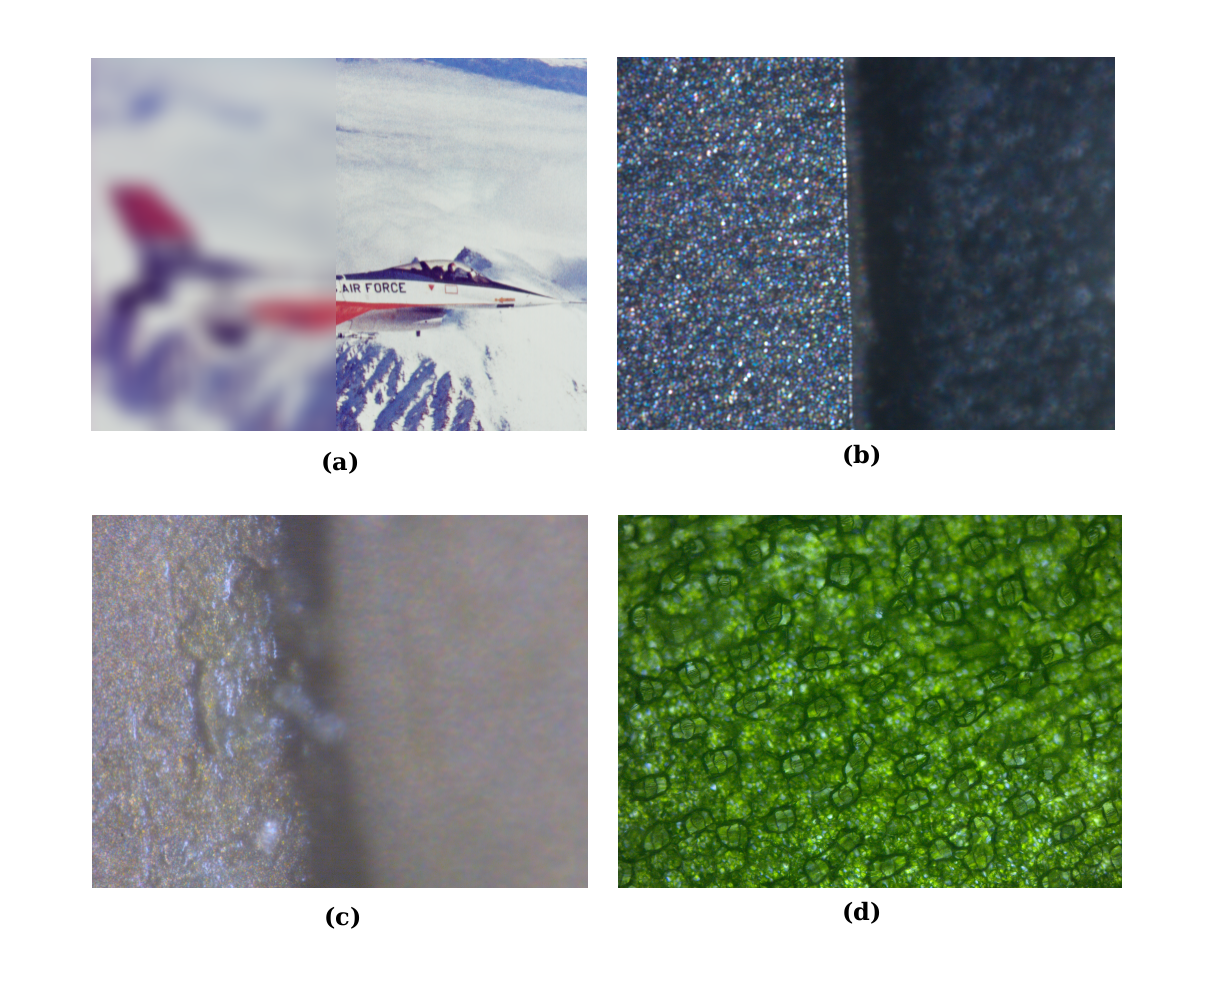
\includegraphics[scale=0.35]{images/fig13.png}
	\end{center}
	\centering
    \fautor
\end{figure}

The images will be acquired with a ZEISS SteREO Discovery.v20 stereo compound microscope. This microscope is used for three-dimensional observations of small objects, with applications in biology, medicine and tissue examination \cite{stereo2012carl}. Figure \ref{fig:stereo_v20} illustrates a stereo compound light microscope from the SCG group that was used to obtain images \ref{fig:validation_images}.\textbf{(b)}, \ref{fig:validation_images}.\textbf{(c) }and \ref{fig:validation_images}.\textbf{(d)}.

\begin{figure}[H]
	\centering
	\caption{\label{fig:stereo_v20}Zeiss SteREO v20 microscope from the SCG group.}
	\begin{center}
	    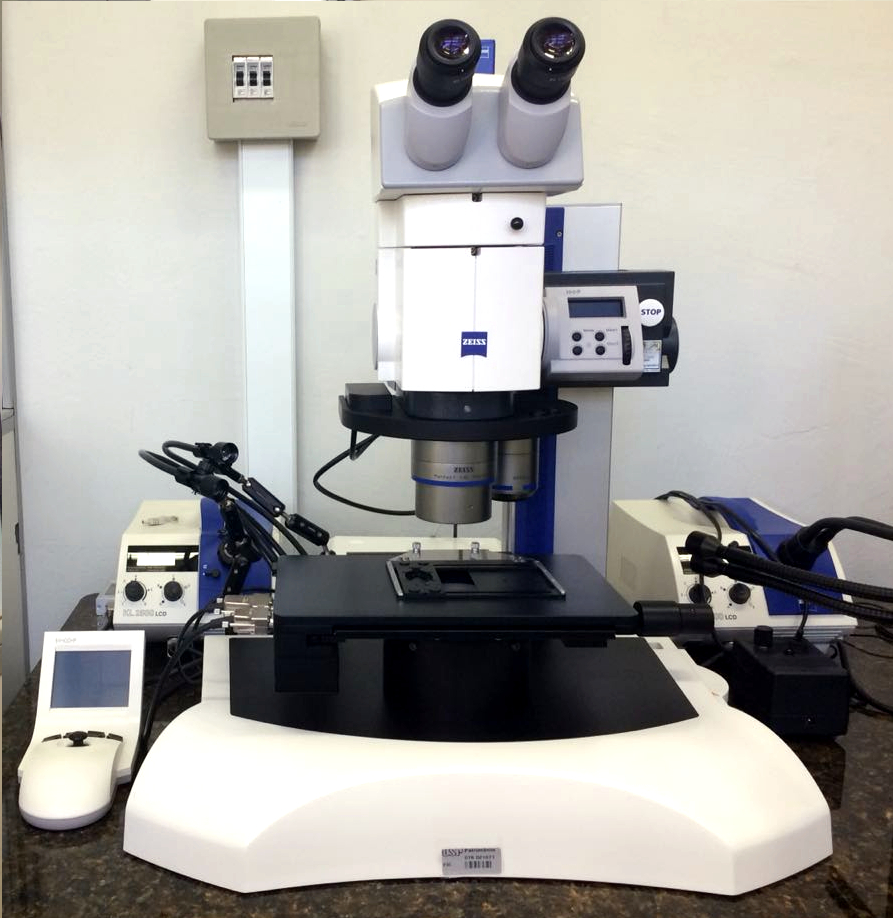
\includegraphics[scale=0.3]{images/fig14.png}
	\end{center}
	\centering
    \fautor
\end{figure}

\section{Methods}

One of the pre-processing tasks consists of colour space conversion, from RGB to HSV and LAB , or to grayscale for testing purposes only. A noise reduction procedure may also be necessary, since microscopy images have a considerable amount of noise. If the amount of noise is created by the texture of the surface, e.g. the coin surface, which shows a particle pattern when magnified, noise reduction procedures should not be done as pre-processing.

According to the literature review from chapter \ref{chapter:related-work}, both segmentation and fusion procedures depend on the problem and should have their parameters optimized empirically. There are several approaches applied by image segmentation algorithms such as pixel-level analysis, region based segmentation, edge based segmentation and so on. Those which are done in the spatial domain have a high computational cost and also a high computational complexity, and are designed for tasks where the segmentation appears to be simple. For region-based segmentation, there are techniques that rely on other mathematical frameworks, e.g. transform domain methods, statistical analysis and linear algebra, as shown in chapter \ref{chapter:related-work}. This work proposes a region-based image segmentation method within transform domains.

The first proposed method for blur segmentation lies upon FFT analysis to identify images with low degree of blur. The most trivial method to be tested is the computation of spectral energy density in frequency bands of the global FFT. The energy in this contexts is somehow related to its concept is physics: the amount of some quantity that should be transferred to something in order to promote the increase or decrease of some property, e.g. the transfer of heat in order to increase the temperature. In this case, spectral energy density consists of the frequency response of the amount of photons which were transferred to the sensor when the image was acquired. The energy can be computed with the $L_{2}$ norm as described in equation \ref{eqn:spectral_energy_density}:

\begin{equation}
\label{eqn:spectral_energy_density}  
    E = \sum_{x=0}^{M-1}\sum_{y=0}^{N-1}|F(x,y)|^{2}
\end{equation}

\noindent where $F$ is the FFT coefficients from the transformed image, $M$ and $N$ are the dimensions of the spectrum. The frequency bands, considering the shift of smallest coefficients to the center of the spectrum, the center as an origin for a coordinate system and the image dimensions as $N$x$N$, consists of lower frequencies in circles around the center (with radius $r < N/2$), medium frequencies when $r$ is close to $N/2$ and high frequencies when $r > N/2$. The idea is that blurry images have spectral energy density values with lower magnitudes, since the blurring process promotes a loss of details and is similar to low-pass filtering operation.

The acquisition of the different bands in two-dimensional spectra can be made with circles centered at the zero frequency, shifted to the image central coordinate. Alternatively, the use of rectangles (or frames) may have similar effects due to the fact that the spectrum can be taken as a mixture of two one-dimensional spectra in each axis. In the end of the process,  images can be taken as sharp or blurry, considering the magnitude of the energy values.

Following this approach, the next trial is to apply the two-dimensional STFT and also compute the energy in different bands. It is known that microscopy images suffer partial blur due to the depth of field feature. Therefore, local analysis may be used to obtain a precise blur map. The algorithm for computing the transform consists of the following steps:

\begin{enumerate}[label=\Roman*.]
    \item Generate a discrete two-dimensional window from two one-dimensional windows. The lengths of each window are taken as input, but it is mandatory that their dimensions originate a window that fits into the image;
    
    \item Separate the image in slices of the same dimensions of the window. For each slice, perform the inner product between the image and the window;
    
    \item For each windowed slice, perform the FFT.
\end{enumerate}

The result is a set of local FFTs. For blurred slices, higher energy values within the low--mid bands will be expected. 

The next step is the image fusion. According to \citeonline{garg2014survey}, the spatial domain-based algorithms cause blur and are sensitive to noise, but contain reasonable information about positions of objects in the scene. Transform domain-based solutions are more complex to implement and also have a higher computational complexity in comparison its counterpart. Therefore, transform domain techniques alone, or a combination of both,  is suitable for this work.

The proposed image fusion algorithm is based on the Fourier domain. Since the proposed segmentation procedure provides a blur map and transforms the image from the spatial domain to the Fourier domain, it is possible to use the information of the blur maps and also the remaining coefficients from the transform in order to perform image fusion. Considering that each coefficient represents a pixel in the original image, the image slices from the STFT on each of the multifocus images can be considered as a \emph{tensor} (a higher dimension array in this case). Figure \ref{fig:tensor} denotes a simple example of the tensor concept:

\begin{figure}[H]
	\centering
	\caption{\label{fig:tensor}Graphical idea of a $8$x$8$x$8$ tensor, which arbitrarily represents the structure of the blur maps and the resulting Fourier spectra from the segmentation procedure.}
	\begin{center}
	    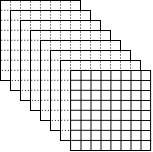
\includegraphics[scale=0.8]{images/fig15.png}
	\end{center}
	\centering
    \fautor
\end{figure}

\noindent For each pixel of the image, which corresponds to one complex coefficient in one of the Fourier spectra, the average of the values should be calculated and the coefficient with the highest similarity will be chosen as the corresponding pixel to compose the fused image. If a set of coefficients has the same similarity when compared to the average value, it means that all related pixels have the same degree of sharpness, then the coefficient may be randomly chosen. 




\section{Evaluation Methods}

According to \citeonline{bovik2009mean}, the \sigla{MSE}{Mean Squared Error} is a measure of signal fidelity. Two signals are compared and a quantitative measure that describes the degree of similarity (fidelity), or the degree of error between them is computed. One indicator is considered as ideal and the other as a result of processes that may have distortions and inconsistencies. Considering $f (x, y)$ and $g (x, y)$ as two functions, the MSE can be represented by the equation \ref{eqn:mse}, and in a general way by equation \ref{eqn:mse_lp_norm}:

\begin{equation}
\label{eqn:mse}
	MSE =  \frac{1}{MN}\sum_{i=1}^{M}\sum_{j=1}^{N}(f(x,y) - g(x,y))^2
\end{equation}

\begin{equation}
\label{eqn:lp_norm2}
	d_p(f,g) = \Bigg(\sum_{i=1}^{M}\sum_{j=1}^{N}|f(x,y) - g(x,y)|^{p}\Bigg)^{1/p}
\end{equation}

\begin{equation}
\label{eqn:mse_lp_norm}
	MSE =  \frac{1}{MN}d_p(f,g)
\end{equation}

\noindent where $M$ and $N$ are the dimensions of both signals and $p$ is the $l_{p}$ norm value, defined as distance function $d:S$ x $S \rightarrow \mathbb{R}^2$. An important derivation of this measure is the RMSE, which is just the root square of the MSE value and changes the range of the metric. For image processing, the MSE is converted into the PSNR metric, which is defined by the equation \ref{eqn:psnr}:

\begin{equation}
\label{eqn:psnr}
	PSNR = 10\log_{10}\Bigg(\frac{L^2}{\sqrt{MSE}}\Bigg)
\end{equation}

\noindent where $L$ is the intensity range for each pixel, usually $[0,255]$.

The resulting blur map from the segmentation process is an array with binary values; it is possible to quantitatively determine the reliability of the segmentation. According to \citeonline{choi2009survey}, the binary feature vector is one of the most common pattern representations, and the similarity and distance measures performed in these sets of information are important for grouping, sorting and analysing data.

Two common similarity metrics, the Jaccard and Dice indices, are appropriate in this scenario. Both are comprised within the $[0,1]$ interval, where 1 is the complete similarity and 0 the complete discrepancy. Table \ref{tab:jaccard_contingency} represents the relationship between the presence and absence of the pixels in two sets A (ground truth segmentation) and B (segmented image).

        \begin{table}[!hbt]
		% Center the table
		\begin{center}
		% Title of the table
		\caption{Contingency table for Jaccard and Dice similarity indices.}
		\label{tab:jaccard_contingency}
		% Table itself: here we have two columns which are centered and have lines to the left, right and in the middle: |c|c|
		\begin{tabular}{|c|c|c|c|}
			% To create a horizontal line, type 
            \hline
             & Presence (A) & Absence (A) & $\mathit{\sum}$\\
    		\hline
          	 Presence (B) & a & b & a + b\\
    		\hline
          	 Absence (B) & c & d & c + d\\
			\hline
             $\mathit{\sum}$ & a + c & b + d & a + b + c + d\\
            \hline
		\end{tabular}
		\end{center}
		\fautor
      \end{table}
      
In this work, $a$ is the number of pixels classified as blurred in both sets, $b$ is the number of pixels classified as blurred in B but not in A, $c$ is the number of pixels classified as blurred in A but not in B, and $d$ is the number of pixels classified as sharp in both sets. As a result, the Jaccard and Dice similarity indices can be described by the equations \ref{eqn:jaccard} and \ref{eqn:dice}, respectively:

\begin{equation}
\label{eqn:jaccard}
	S_{jaccard} = \frac{a}{a + b + c}
\end{equation}

\begin{equation}
\label{eqn:dice}
	S_{dice} = \frac{2a}{2a + b + c}
\end{equation}

\chapter{Preliminary Results}
\label{chapter:preliminary-results}
Experiments for the segmentation procedure were carried out for the two proposed methods: a) FFT and b) STFT. The proposed image sets were built in order to perform tests with real multifocus microscopy images with their own point spread function and defocus blur feature. The coin images were acquired with 300x magnification,  5 $\mu m$ Depth of Field and 10 $\mu m$ step between each image on the $z$ axis. Two different slopes between the coin letters were considered: the slope between the background of the coin and the "o" letter and the same approach for the 90 degrees rotated "v" letter in the Portuguese word \emph{centavos} of the coin, shown in figure \ref{fig:original_coin}. The slope on the images was made on purpose for creating a very pronounced blur effect with the differences in the microscope objective's height. Ten images were taken from the "o" and "v" slopes. The blurred parts are known to be either \emph{left} or \emph{right}, as summarized by table \ref{tab:coin_card_set_description} and shown in figure \ref{fig:card_coin_images}:

\begin{figure}[H]
	\centering
	\caption{\label{fig:original_coin}10-\emph{cent} Brazilian Real coin.}
	\begin{center}
	    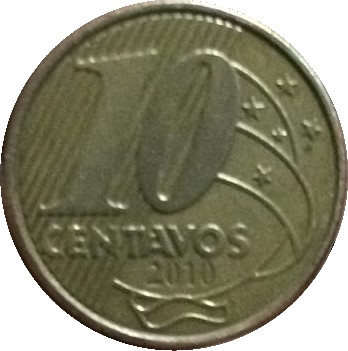
\includegraphics[scale=0.5, trim = {0 0 0 1cm}]{images/fig16.png}
	\end{center}
	\centering
    \fautor
\end{figure}

\begin{table}[H]
    \centering
    \caption{Description of the sharp parts of the image sets (a) coin "o" letter and (b) coin "v" letter.}\label{tab:coin_card_set_description}
    \begin{subtable}{.35\linewidth}
    
    %Center the table
		\begin{center}
		% Title of the table
		\caption{}
        \begin{tabular}
        {|c|c|c|}
        \hline
        
            % header
            Image & Sharp Part
            \\ \hline
            % data
            coin "o" 1 & None
            \\ \hline
            
            coin "o" 2 & None
            \\ \hline
            
            coin "o" 3 & Left
            \\ \hline
            
            coin "o" 4& Left
            \\ \hline
            
            coin "o" 5 & Left
            \\ \hline
            
            coin "o" 6 & Right
            \\ \hline
            
            coin "o" 7 & Right
            \\ \hline
            
            coin "o" 8 & None
            \\ \hline
            
            coin "o" 9 & None
            \\ \hline
            
            coin "o" 10 & None
            \\ \hline
            
        \end{tabular}
    \end{center}
    \end{subtable}%
    \begin{subtable}{.35\linewidth}

        %Center the table
		\begin{center}
		% Title of the table
		\caption{}
        \begin{tabular}
        {|c|c|c|}
        \hline
        
            % header
            Image & Sharp Part
            \\ \hline
            % data
            coin "v" 1 & None
            \\ \hline
            
            coin "v" 2 & None
            \\ \hline
            
            coin "v" 3 & Right
            \\ \hline
            
            coin "v" 4& Right
            \\ \hline
            
            coin "v" 5 & Right
            \\ \hline
            
            coin "v" 6 & Right
            \\ \hline
            
            coin "v" 7 & Left
            \\ \hline
            
            coin "v" 8 & Left
            \\ \hline
            
            coin "v" 9 & Left
            \\ \hline
            
            coin "v" 10 & Left
            \\ \hline
            
        \end{tabular}
    \end{center}
    \end{subtable} 
    \hspace{0.8cm}
    \fautor
\end{table}

\begin{figure}[H]
	\centering
	\caption{\label{fig:card_coin_images}Samples from the coin and card image sets: (a) and (b) left and right sharp sides of coin "o" letter, respectively, (c) and (d) left and right sharp sides of coin "v" letter, respectively.}
	\begin{center}
	    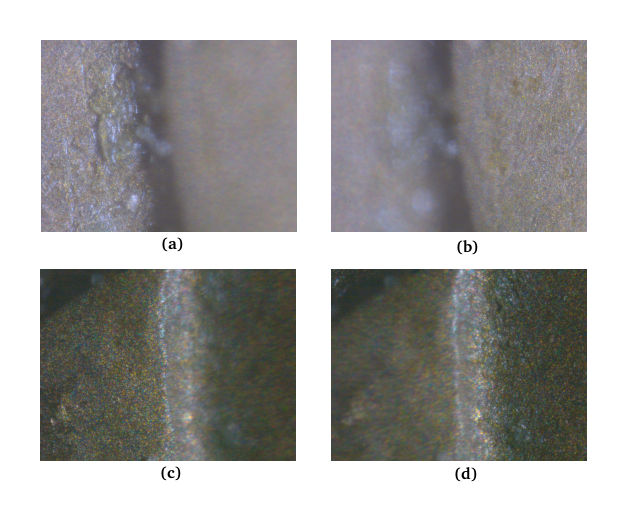
\includegraphics[scale=0.6, trim = {0 1cm 0 1cm}]{images/fig17.png}
	\end{center}
	\centering
    \fautor
\end{figure}

\noindent An analogous image set for testing purposes was created, i.e. the card. It consists of images of a contact pad for the electrical interface of a bank card. It was chosen because of a coarser slope when compared to the coin images. The images were acquired also with 300x magnification, a 5 $\mu m$ Depth of Field and a 10 $\mu m$ step between each image on the $z$ axis. Some samples of the card image set are denote by figure \ref{fig:card_set_images} and the description of the card set can be seen in table \ref{tab:card_set_description}.

\begin{figure}[H]
	\centering
	\caption{\label{fig:card_set_images}Card contact pad images: contact pad (a), left and right sharp sides (b) .}
	\begin{subfigure}{.5\textwidth}
        \centering
        \frame{
\includegraphics[scale=1]{images/fig18a.png}}
        \caption{}
    \end{subfigure}\\
    \begin{subfigure}{\textwidth}
         \centering
         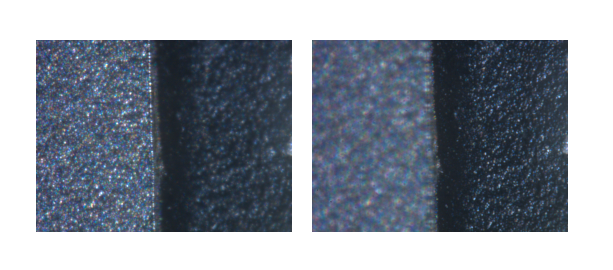
\includegraphics[scale=0.5, trim = {0 0cm 0 0cm}]{images/fig18b.png}
         \caption{}
    \end{subfigure}
	    \fautor
\end{figure}


\begin{table}[htb]
    \centering
    \caption{Description of the sharp parts of the card image set.}\label{tab:card_set_description}
    %Center the table
		\begin{center}
		% Title of the table
        \begin{tabular}
        {|c|c|c|}
        \hline
            % header
            Image & Sharp Part
            \\ \hline
            % data
            card 1 & None
            \\ \hline
            
            card 2 & None
            \\ \hline
            
            card 3 & Left
            \\ \hline
            
            card 4& Left
            \\ \hline
            
            card 5 & Left
            \\ \hline
            
            card 6 & Left
            \\ \hline
            
            card 7 & Right
            \\ \hline
            
            card 8 & Right
            \\ \hline
            
            card 9 & Right
            \\ \hline
            
            card" 10 & Right
            \\ \hline
            
            card" 11 & None
            \\ \hline

            card" 12 & None
            \\ \hline
            
        \end{tabular}
    \end{center}
    \fautor
\end{table}

An artificially blurred image was also used for the tests. The airplane image consists of an common standard $256$x$512$ test image of an F-16 airplane, obtained from the \sigla{USC-SIPI}{University of Southern California - Signal and Image Processing Institute} image databases \cite{uscsipi1977image}. The blurring process consisted of dividing the image in two halves (left and right) with $256$x$512$ pixels each and blurring the left one with a Gaussian Blur Kernel of radius $30$ with the aid of \sigla{GIMP}{GNU Image Manipulation Program}. This image set is shown in figure \ref{fig:airplane_set_images}:

\begin{figure}[H]
	\centering
	\caption{\label{fig:airplane_set_images}Airplane contact pad images: left (a) and right (b) sharp sides.}
	\begin{center}
	    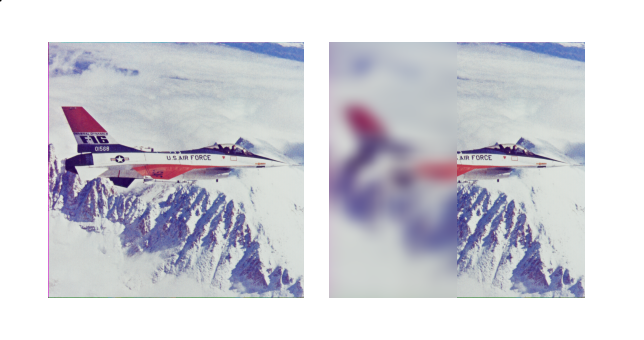
\includegraphics[scale=0.6, trim = {0 1cm 0 1cm}]{images/fig19.png}
	\end{center}
	\centering
    \fautor
\end{figure}

\section{FFT Test}
\label{sec:fft-test}

As expected, the global approach is capable of electing the mostly sharp image within a set of partially blurred images. The magnitude of the spectral energy density values was higher for the sharper images, mostly the ones which have a sharp side, either left or right. Three frequency bands were considered to compute the results: \emph{mid}, \emph{high} and \emph{highest}. The computation of the bands was done in the three proposed colourspaces, and the grayscale one was the most precise. Comprehensive results for grayscale and other colourspaces are shown in appendix \ref{chapter:fft-test-results}. Notice that this approach is not capable of precisely pointing out the location of the blurry parts of the image. Figure \ref{fig:fft_results} presents the frequency band energy values with the grayscale colourspace on each band for the FFT approach. The amount of bar triads is related to the amount of images in the set: for the coin "o" and coin "v" images, 10 bar triads were shown; analogously, 12 for the card set and 2 for the airplane set.

\begin{figure}[H]
    \centering
    \caption{\label{fig:fft_results}Grayscale colourspace FFT approach for coin "o" (upper left), coin "v" (upper right), card (lower left) and airplane (lower right) images.}
    \subfloat{
        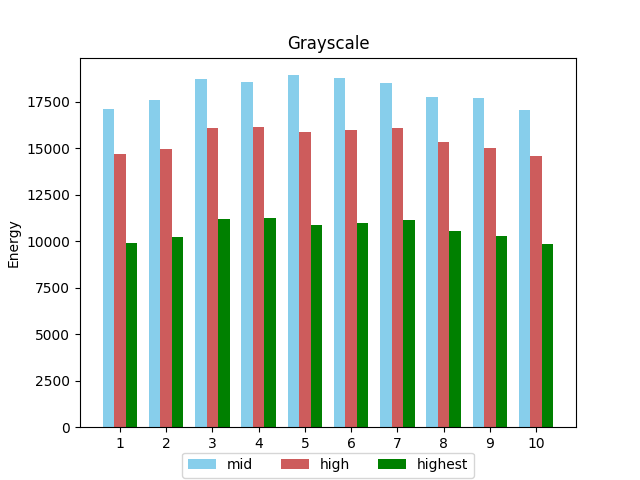
\includegraphics[width=0.45\textwidth]{images/fig20a.png}
        \label{fig:subfig1}
    }
    \qquad
    \subfloat{
        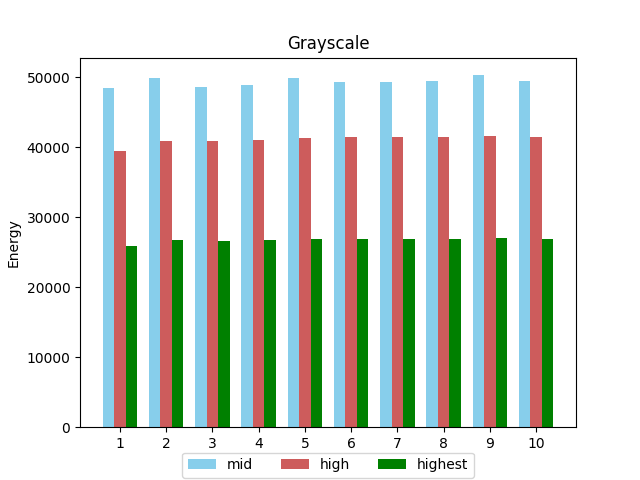
\includegraphics[width=0.45\textwidth]{images/fig20b.png}
        \label{fig:subfig2}
    }
    \subfloat{
        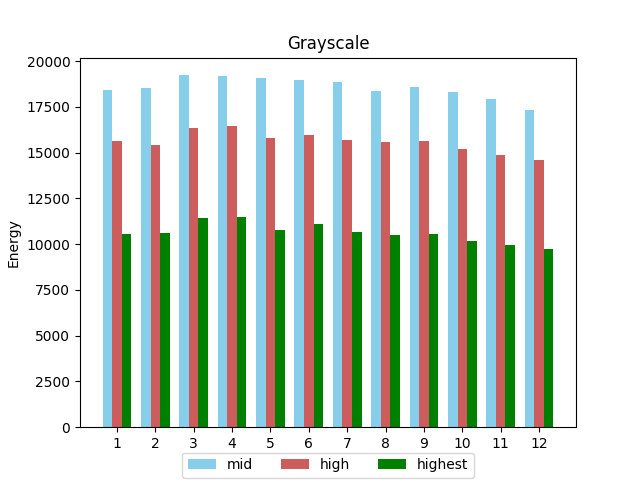
\includegraphics[width=0.45\textwidth]{images/fig20c.png}
        \label{fig:subfig3}
    }
    \qquad
    \subfloat{
        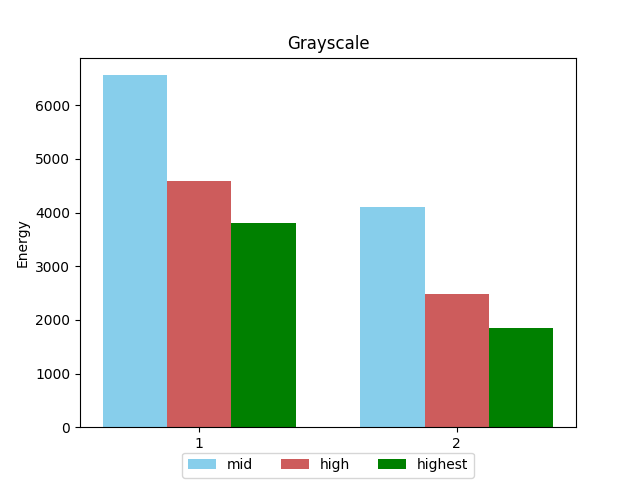
\includegraphics[width=0.45\textwidth]{images/fig20d.png}
        \label{fig:subfig4}
    }
    \hspace{1cm}
    \fautor
\end{figure}

\section{STFT Test}

The Short-time Fourier Transform approach presented relevant results concerning the information about the amount of blur on each region of the images. The test cases were made in such a way that positive results should be expected: the most efficient window size was already set due to the prior knowledge about the blurry and the sharp regions. With the same configuration for colourspaces and frequency bands, the test were done with several different window functions that are printed on the appendix \ref{chapter:stft-test-results}. The figures \ref{fig:stft_card}, \ref{fig:stft_coin_o}, \ref{fig:stft_coin_v} and \ref{fig:stft_airplane} presents the frequency band energy values with the grayscale colourspace on each band for the STFT approach, with the Hann window function, for the left and right sections (left and right in the airplane graph and \emph{L} and \emph{R} for the other graphs). The graphs stand for the card, coin "o", coin "v" and airplane image sets, respectively. The bar triad settings are the same as in section \ref{sec:fft-test}.


\begin{figure}[ht]
	\centering
	\caption{\label{fig:stft_card}Grayscale colourspace STFT approach for card images.}
	\begin{center}
	    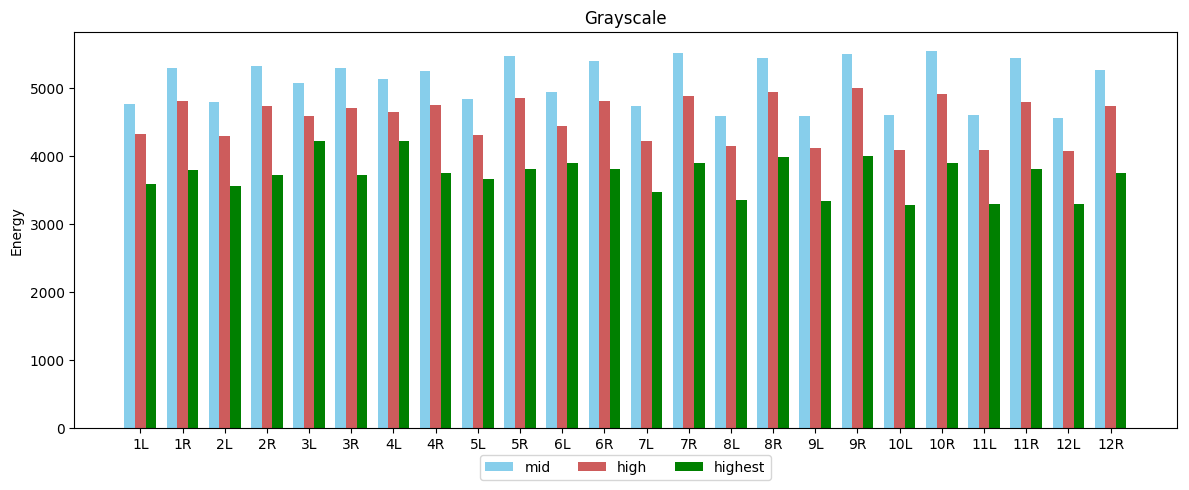
\includegraphics[scale=0.52, trim = {0 1cm 0 1cm}]{images/fig21.png}
	\end{center}
	\centering
    \fautor
\end{figure}

\begin{figure}[ht]
	\centering
	\caption{\label{fig:stft_coin_o}Grayscale colourspace STFT approach for coin "o" images.}
	\begin{center}
	    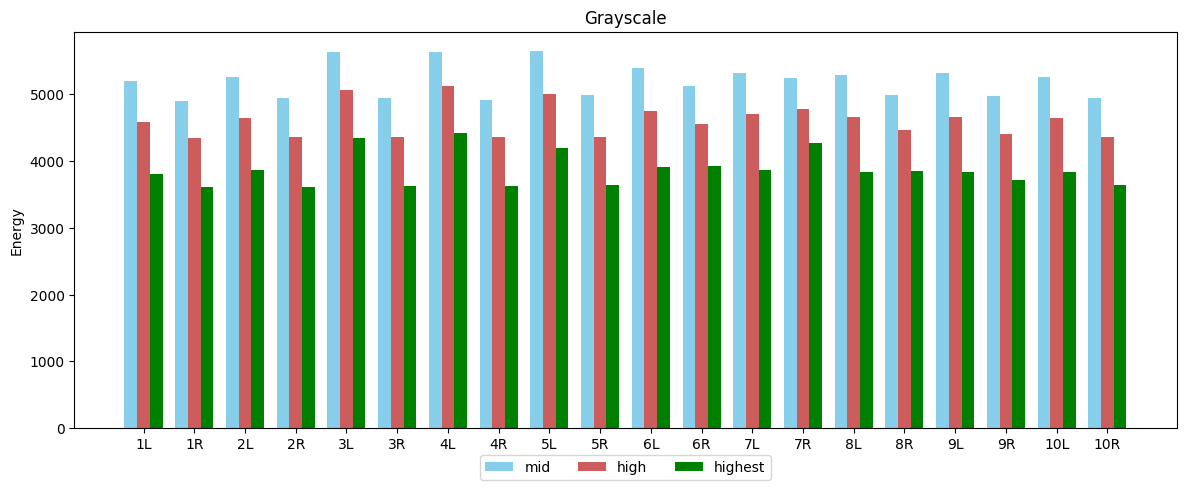
\includegraphics[scale=0.52, trim = {0 1cm 0 1cm}]{images/fig22.png}
	\end{center}
	\centering
    \fautor
\end{figure}

\begin{figure}[ht]
	\centering
	\caption{\label{fig:stft_coin_v}Grayscale colourspace STFT approach for coin "v" images.}
	\begin{center}
	    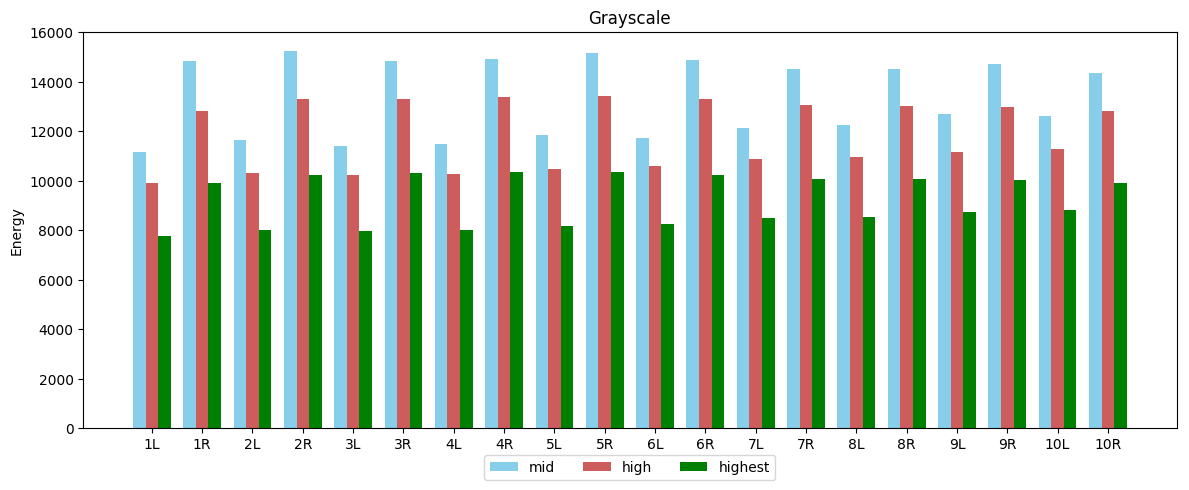
\includegraphics[scale=0.52, trim = {0 1cm 0 1cm}]{images/fig23.png}
	\end{center}
	\centering
    \fautor
\end{figure}

\begin{figure}[ht]
	\centering
	\caption{\label{fig:stft_airplane}Grayscale colourspace STFT approach for airplane images.}
	\begin{center}
	    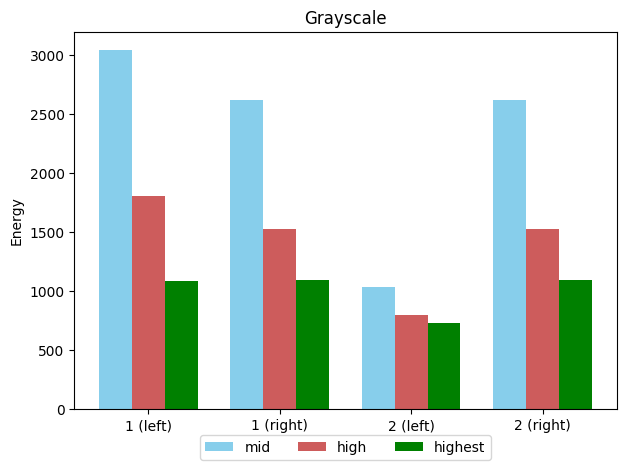
\includegraphics[scale=0.6, trim = {0 1cm 0 1cm}]{images/fig24.png}
	\end{center}
	\centering
    \fautor
\end{figure}

\noindent The above graphs show that the magnitude of the energy levels on blurry sections is lower than the same metric for the non-blurry ones. Therefore, it provides evidence about the blur location. The most relevant results were obtained with the Grayscale and HSV colourspaces, such that neither the appendix \ref{chapter:fft-test-results} nor the \ref{chapter:stft-test-results} show the LAB results.

\chapter{Conclusions}
\label{chapter:conclusions}
From the preliminary results, it is possible to envisage and plan the activities to be done during the year of 2019 in order to achieve better performances and also better results. Preparations for the qualification exam and took consumed most of January and February. During this period, adjustments in the code were made and the necessity of some changes was noticed. These will be implemented and tested in March and April, together with the development of scientific articles with the proposed methods and results. After some changes in the code, improvements in the methods and evaluation of the tests, the new achievements should be summarized into the thesis; this will be done in May, June and July. More improvements may be done if needed during August and September, together with the article writing step. The last three months will be dedicated to prepare the thesis and to the defense. This schedule program is graphically represented in table \ref{tab:activity_schedule}:

\begin{table}[H]
    \caption{Activity schedule for 2019.}\label{tab:activity_schedule}
    \begin{center}
    \begin{tabular}{|c|c|c|c|c|c|c|c|c|c|c|c|c|}
        \hline
   
        & \multicolumn{6}{c|}{$1^{st}$ semester} 
        & \multicolumn{6}{c|}{$2^{nd}$ semester}\\
        \hline
   
        & jan & feb & mar & apr & may & jun 
        & jul & aug & sep & oct & nov & dec\\
        \hline
        
        Qualification
        & \cellcolor{gray} & \cellcolor{gray} &  &  &  &  
        &  &  &  &  &  & \\
        \hline
        
        Paper / Code
        &  & \cellcolor{gray} & \cellcolor{gray} & \cellcolor{gray} &  & &  &  &  &  &  & \\
        \hline
        
        Paper / Thesis
        &  &  &  &  & \cellcolor{gray} & \cellcolor{gray} & \cellcolor{gray} &  &  &  &  & \\
        \hline
        
        Paper / Code
        &  &  &  &  & &  &  & \cellcolor{gray} & \cellcolor{gray} &  &  & \\
        \hline
        
        Thesis
        &  &  &  &  & &  &  &  &  & \cellcolor{gray} & \cellcolor{gray} & \\
        \hline
        
        Defense
        &  &  &  &  & &  &  &  &  &  &  & \cellcolor{gray}\\
        \hline
    \end{tabular}
    \end{center}
    \fautor
\end{table}

% \chapter{Ferramentas úteis}
% \label{chapter:ferramentas-uteis}
% \input{tex/ferramentas-uteis}

% \chapter{Citações e referências}
% \label{chapter:citacoes}
% \input{tex/citacoes}


% ---
% Finaliza a parte no bookmark do PDF, para que se inicie o bookmark na raiz
% ---
\bookmarksetup{startatroot}% 
% ---

% ----------------------------------------------------------
% ELEMENTOS PÓS-TEXTUAIS
 ----------------------------------------------------------
\postextual

% ----------------------------------------------------------
% Referências bibliográficas
% ----------------------------------------------------------
\bibliography{references}

% ---------------------------------------------------------------------
% GLOSSÁRIO
% ---------------------------------------------------------------------

% Arquivo que contém as definições que vão aparecer no glossário
\input{tex/glossario}
% Comando para incluir todas as definições do arquivo glossario.tex
\glsaddall
% Impressão do glossário
\printglossaries

% ----------------------------------------------------------
% Apêndices
% ----------------------------------------------------------

% ---
% Inicia os apêndices
% ---
\begin{apendicesenv}

    \chapter{FFT Results}
    \label{chapter:fft-test-results}
    \begin{figure}[htp]
    \caption{\label{fig:appendix_airplane_fft_results}Airplane FFT approach for (a) Grayscale, (b) HSV and (c) LAB images.}
    \centering
    \begin{subfigure}{.5\textwidth}
        \centering
        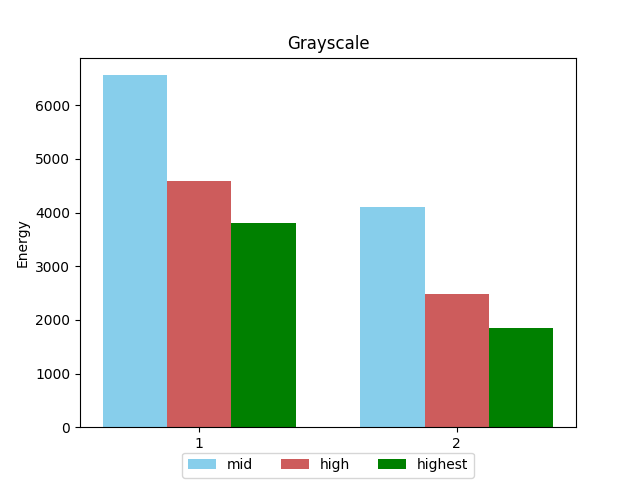
\includegraphics[scale=0.41]{images/appendix/fft/airplane/grayscale.png}
        \caption{}
    \end{subfigure}%
    \begin{subfigure}{.5\textwidth}
         \centering
          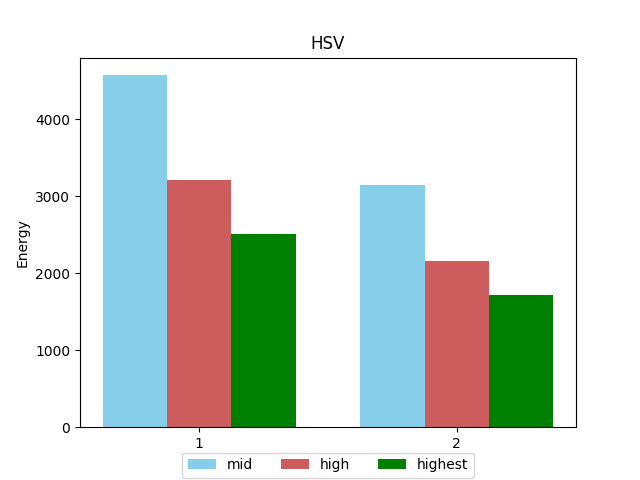
\includegraphics[scale=0.41]{images/appendix/fft/airplane/hsv.png}
          \caption{}
    \end{subfigure}
    \fautor
\end{figure}

\begin{figure}[H]
    \caption{\label{fig:appendix_card_fft_results}Card FFT approach for (a) Grayscale, (b) HSV and (c) LAB images.}
    \centering
    \begin{subfigure}{.5\textwidth}
        \centering
        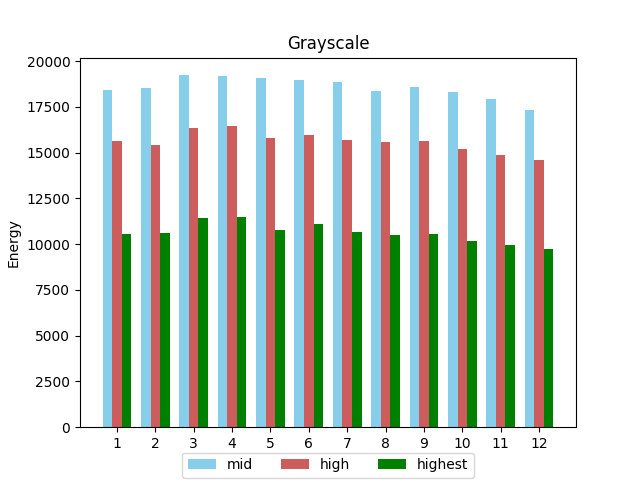
\includegraphics[scale=0.41]{images/appendix/fft/card/grayscale.png}
        \caption{}
    \end{subfigure}%
    \begin{subfigure}{.5\textwidth}
         \centering
          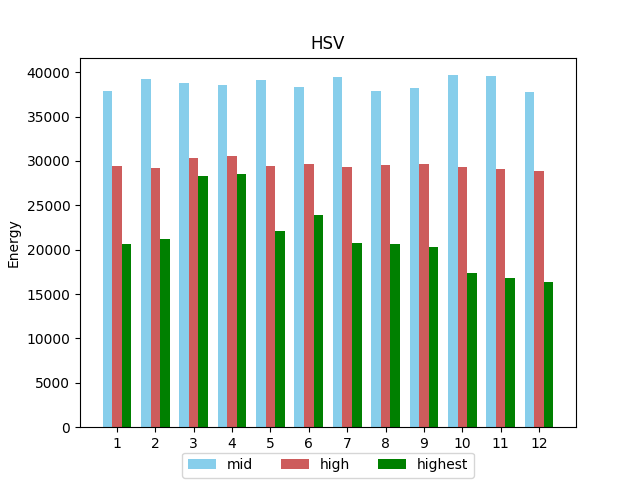
\includegraphics[scale=0.41]{images/appendix/fft/card/hsv.png}
          \caption{}
    \end{subfigure}
    \fautor
\end{figure}

\begin{figure}[H]
    \caption{\label{fig:appendix_coin_o_fft_results}Coin "o" letter FFT approach for (a) Grayscale, (b) HSV and (c) LAB images.}
    \centering
    \begin{subfigure}{.5\textwidth}
        \centering
        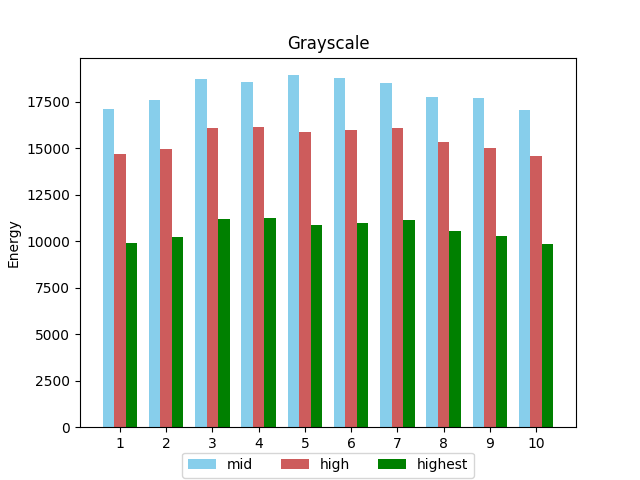
\includegraphics[scale=0.41]{images/appendix/fft/coin_o/grayscale.png}
        \caption{}
    \end{subfigure}%
    \begin{subfigure}{.5\textwidth}
         \centering
          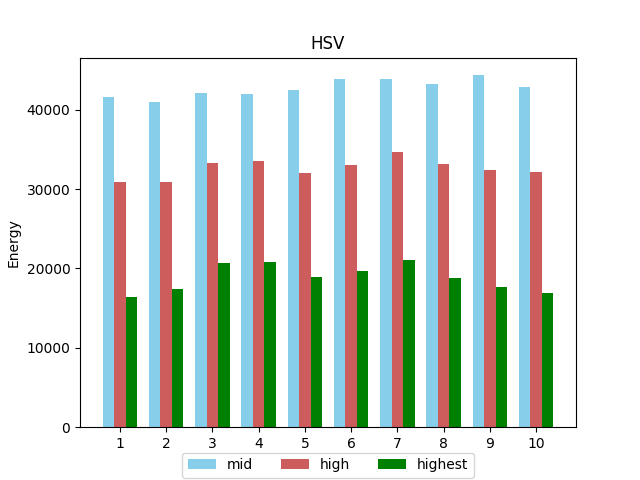
\includegraphics[scale=0.41]{images/appendix/fft/coin_o/hsv.png}
          \caption{}
    \end{subfigure}
    \fautor
\end{figure}

\begin{figure}[H]
    \caption{\label{fig:appendix_coin_v_fft_results}Coin "v" letter FFT approach for (a) Grayscale, (b) HSV and (c) LAB images.}
    \centering
    \begin{subfigure}{.5\textwidth}
        \centering
        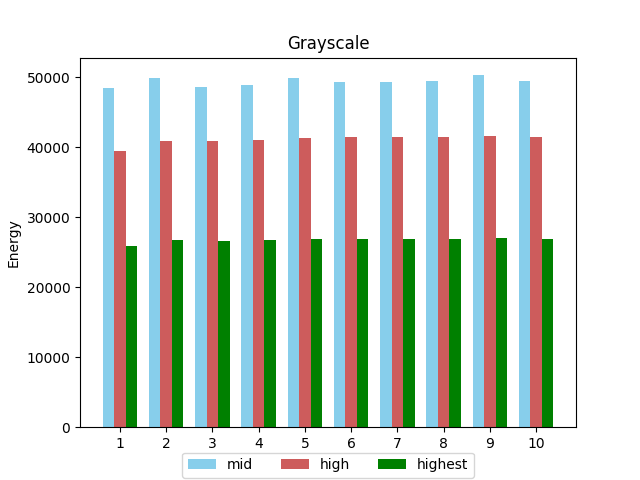
\includegraphics[scale=0.41]{images/appendix/fft/coin_v/grayscale.png}
        \caption{}
    \end{subfigure}%
    \begin{subfigure}{.5\textwidth}
         \centering
          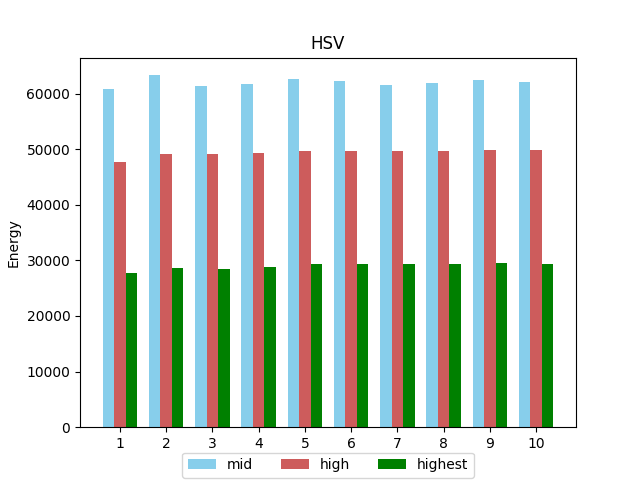
\includegraphics[scale=0.41]{images/appendix/fft/coin_v/hsv.png}
          \caption{}
    \end{subfigure}
    \fautor
\end{figure}

    
    \chapter{STFT Results}
    \label{chapter:stft-test-results}
    \section{Hann Window}

\begin{figure}[!ht]
    \caption{Coin "o" STFT approach with Hann window for Grayscale (a) and HSV (b) colourspaces.}
    \centering
    \begin{subfigure}{\textwidth}
        \centering
        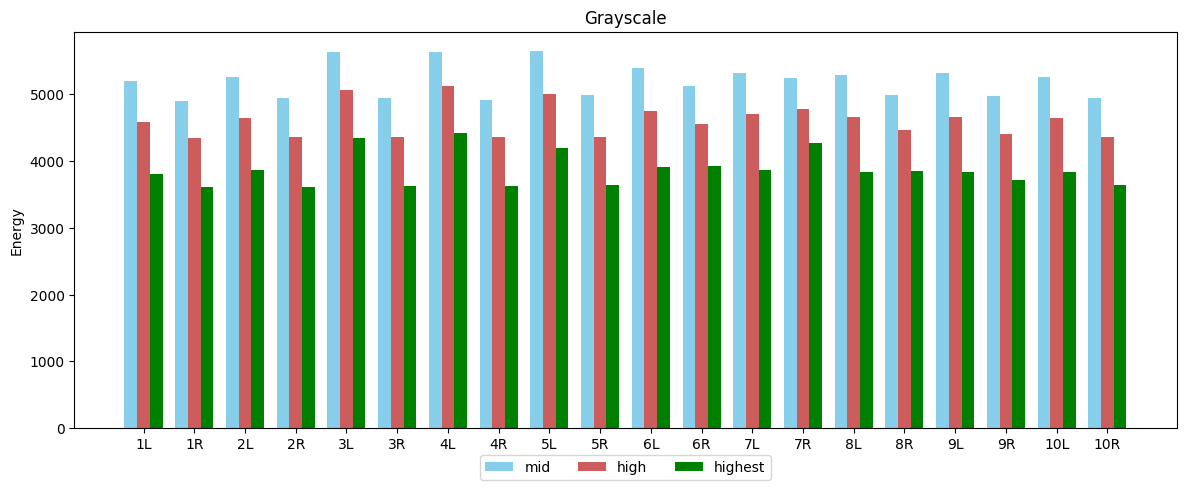
\includegraphics[scale=0.4]{images/appendix/stft/coin_o/hann_Grayscale.png}
        \caption{}
    \end{subfigure}\\
    \begin{subfigure}{\textwidth}
         \centering
          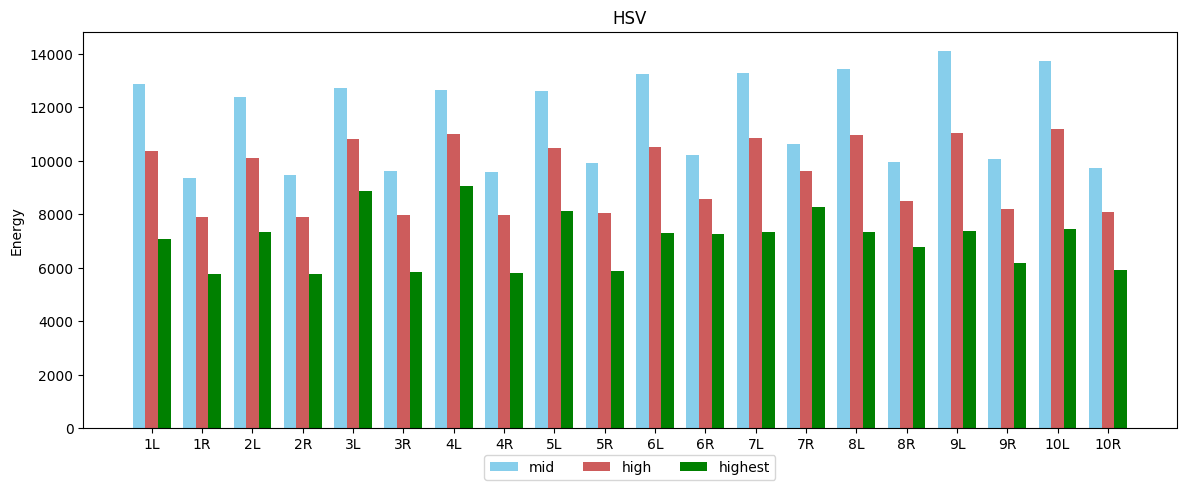
\includegraphics[scale=0.4]{images/appendix/stft/coin_o/hann_HSV.png}
          \caption{}
    \end{subfigure}
    \fautor
\end{figure}

\begin{figure}[H]
    \caption{Card STFT approach with Hann window for Grayscale (a) and HSV (b) colourspaces.}
    \centering
    \begin{subfigure}{\textwidth}
        \centering
        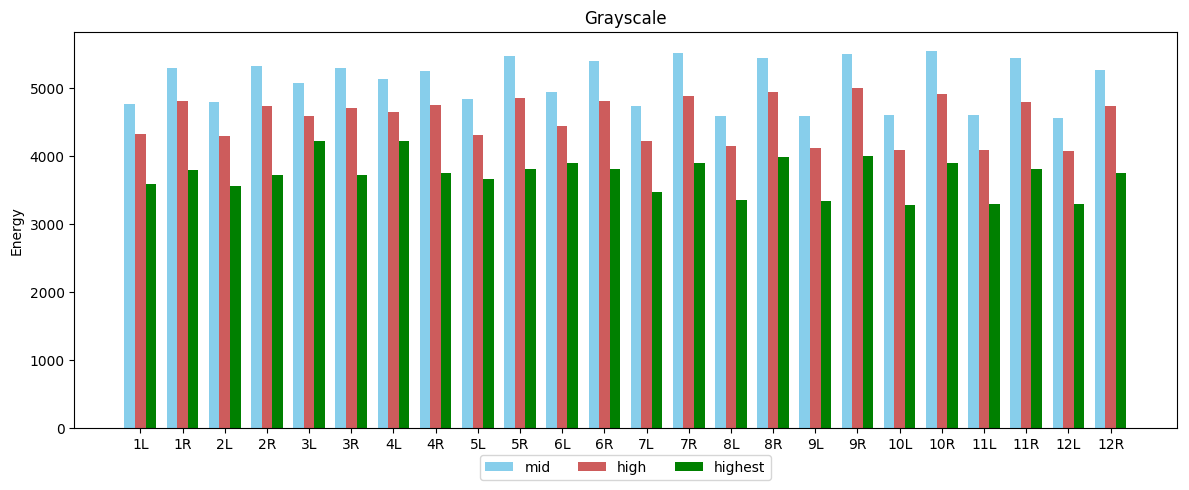
\includegraphics[scale=0.5]{images/appendix/stft/card/hann_Grayscale.png}
        \caption{}
    \end{subfigure}\\
    \begin{subfigure}{\textwidth}
         \centering
          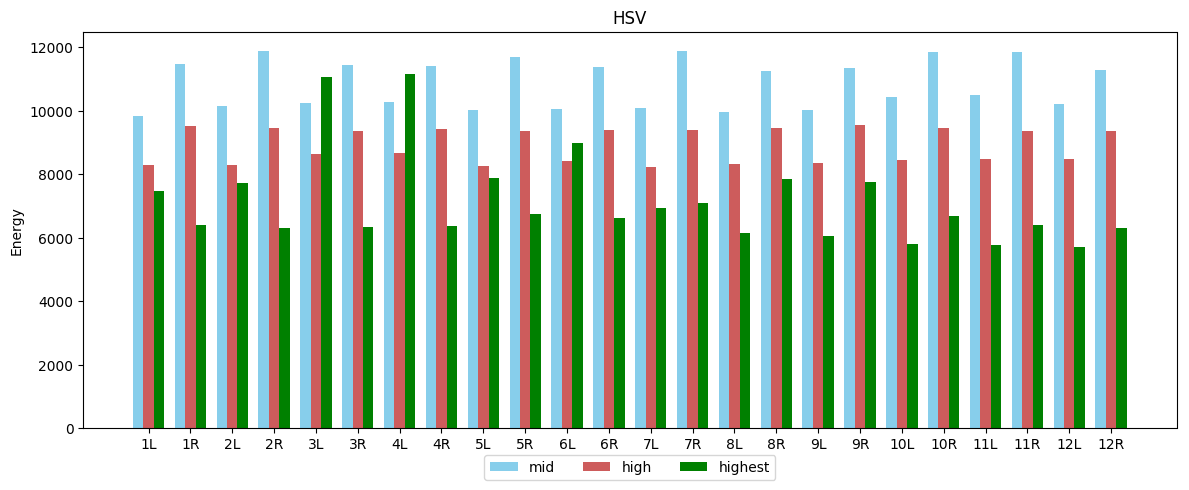
\includegraphics[scale=0.5]{images/appendix/stft/card/hann_HSV.png}
          \caption{}
    \end{subfigure}
    \fautor
\end{figure}

\begin{figure}[H]
    \caption{Airplane STFT approach with Hann window for Grayscale (a) and HSV (b) colourspaces.}
    \centering
    \begin{subfigure}{.5\textwidth}
        \centering
        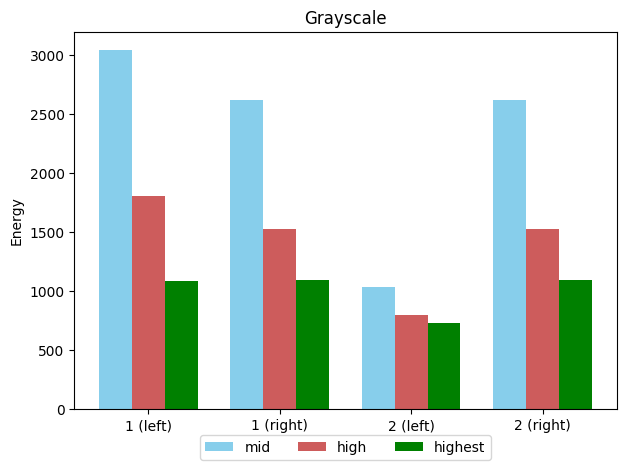
\includegraphics[scale=0.41]{images/appendix/stft/airplane/hann_Grayscale.png}
        \caption{}
    \end{subfigure}%
    \begin{subfigure}{.5\textwidth}
         \centering
          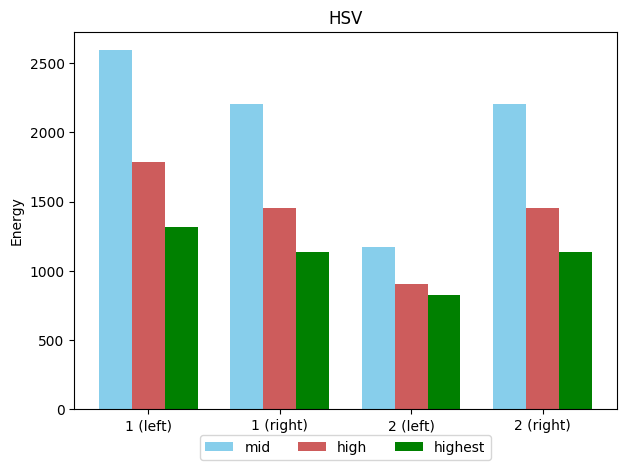
\includegraphics[scale=0.41]{images/appendix/stft/airplane/hann_HSV.png}
          \caption{}
    \end{subfigure}
    \fautor
\end{figure}


\begin{figure}[H]
    \caption{Coin "v" STFT approach with Hann window for Grayscale (a) and HSV (b) colourspaces.}
    \centering
    \begin{subfigure}{\textwidth}
        \centering
        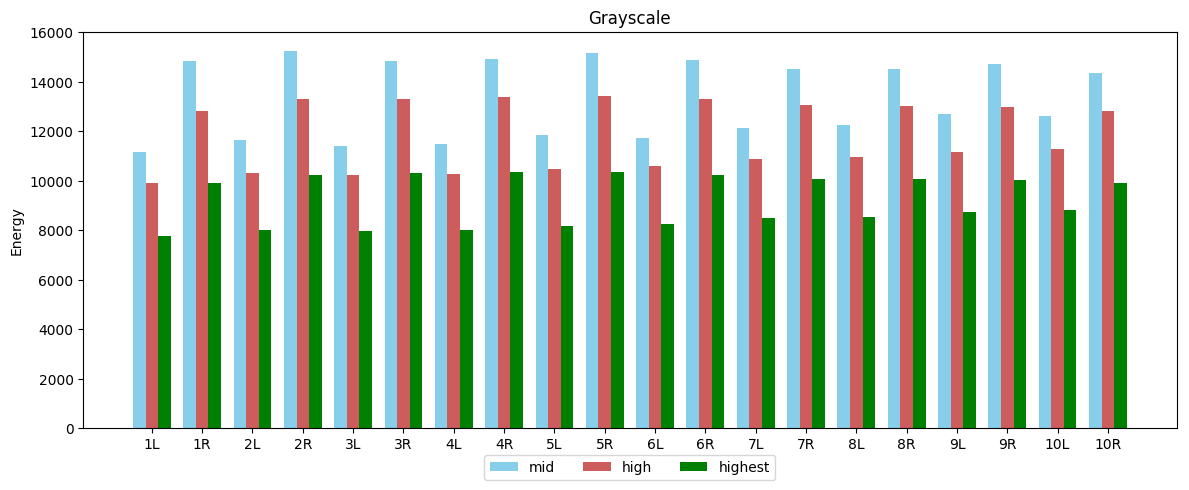
\includegraphics[scale=0.5]{images/appendix/stft/coin_v/hann_Grayscale.png}
        \caption{}
    \end{subfigure}\\
    \begin{subfigure}{\textwidth}
         \centering
          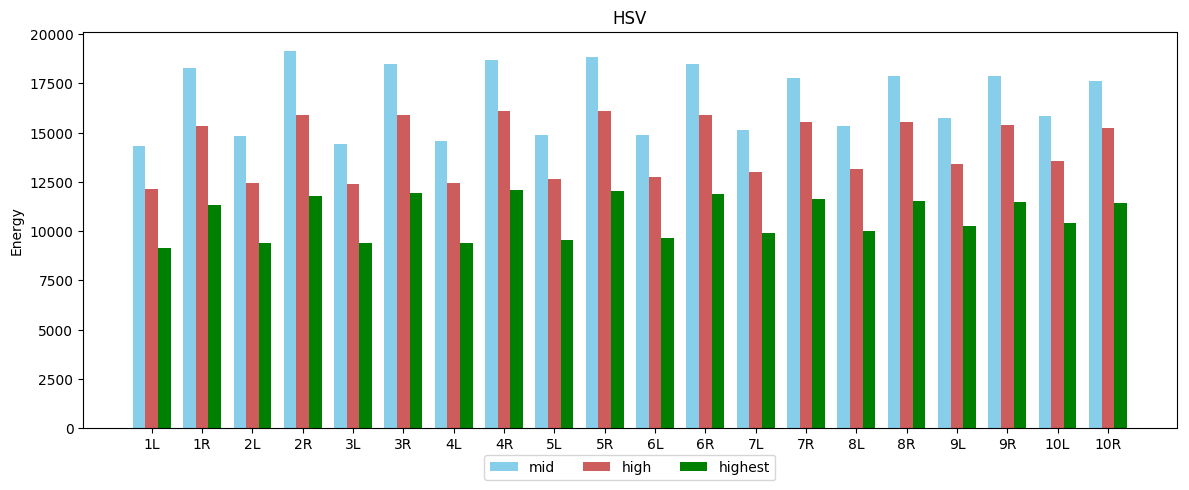
\includegraphics[scale=0.5]{images/appendix/stft/coin_v/hann_HSV.png}
          \caption{}
    \end{subfigure}
    \fautor
\end{figure}

\section{Flattop Window}

\begin{figure}[H]
    \caption{Airplane STFT approach with Flattop window for Grayscale (a) and HSV (b) colourspaces.}
    \centering
    \begin{subfigure}{.5\textwidth}
        \centering
        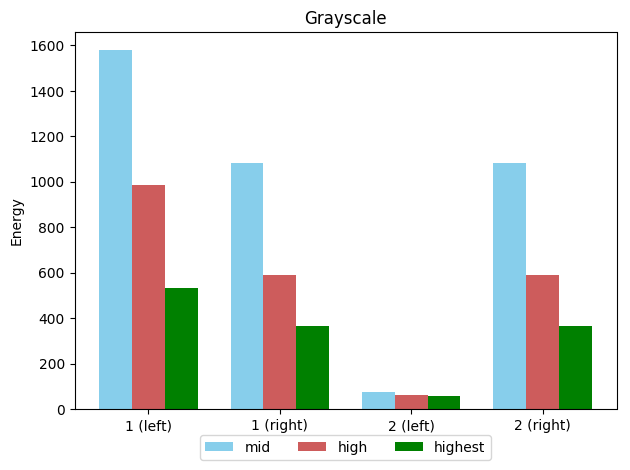
\includegraphics[scale=0.41]{images/appendix/stft/airplane/flattop_Grayscale.png}
        \caption{}
    \end{subfigure}%
    \begin{subfigure}{.5\textwidth}
         \centering
          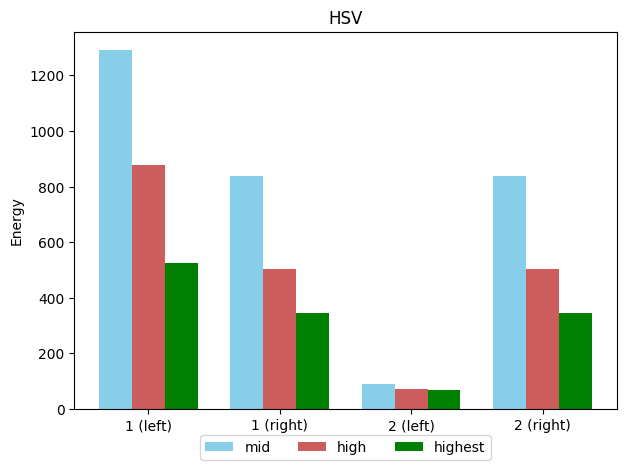
\includegraphics[scale=0.41]{images/appendix/stft/airplane/flattop_HSV.png}
          \caption{}
    \end{subfigure}
    \fautor
\end{figure}

\begin{figure}[!htb]
    \caption{Coin "o" STFT approach with Flattop window for Grayscale (a) and HSV (b) colourspaces.}
    \centering
    \begin{subfigure}{\textwidth}
        \centering
        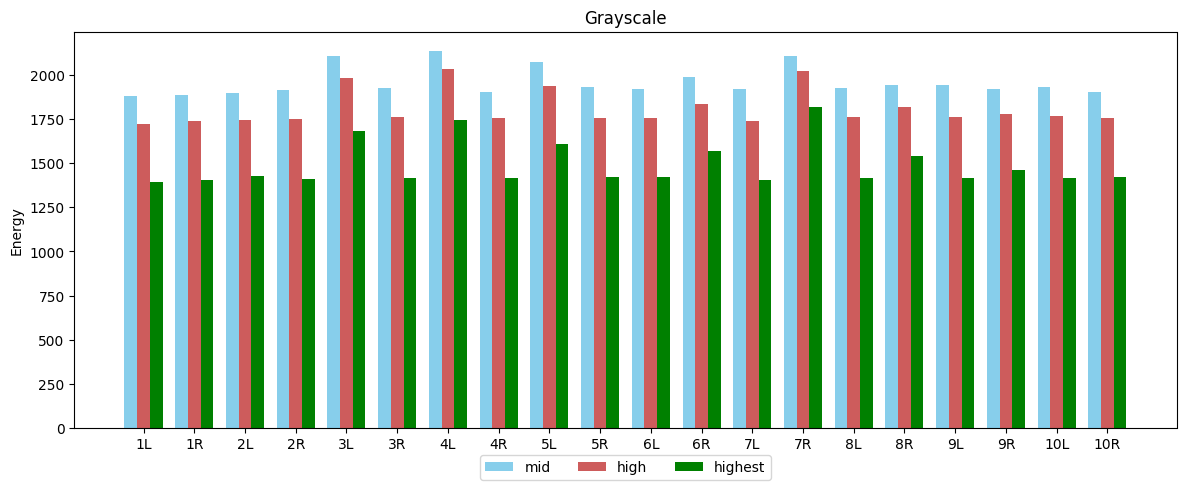
\includegraphics[scale=0.4]{images/appendix/stft/coin_o/flattop_Grayscale.png}
        \caption{}
    \end{subfigure}\\
    \begin{subfigure}{\textwidth}
         \centering
          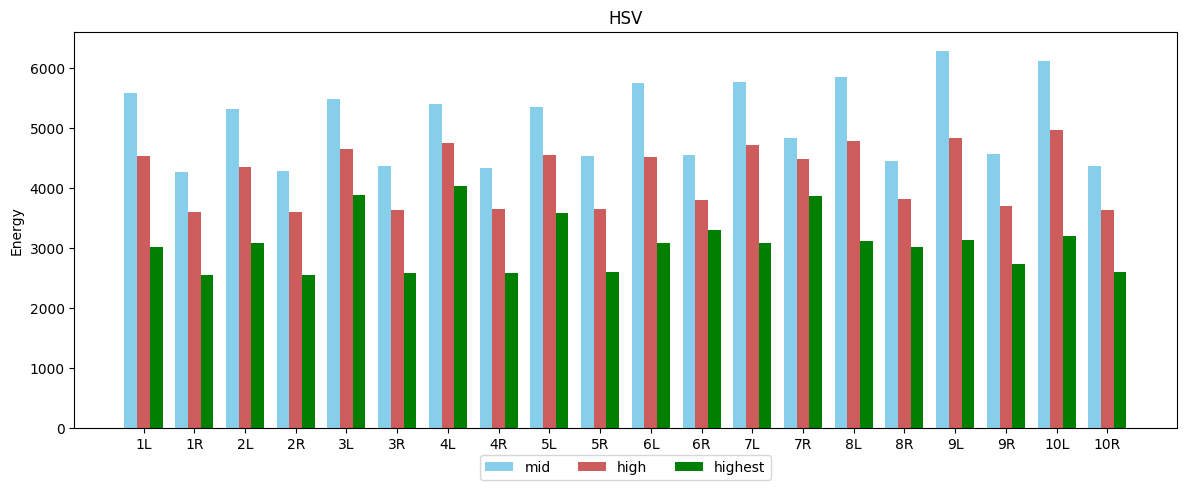
\includegraphics[scale=0.4]{images/appendix/stft/coin_o/flattop_HSV.png}
          \caption{}
    \end{subfigure}
    \fautor
\end{figure}

\begin{figure}[H]
    \caption{Card STFT approach with Flattop window for Grayscale (a) and HSV (b) colourspaces.}
    \centering
    \begin{subfigure}{\textwidth}
        \centering
        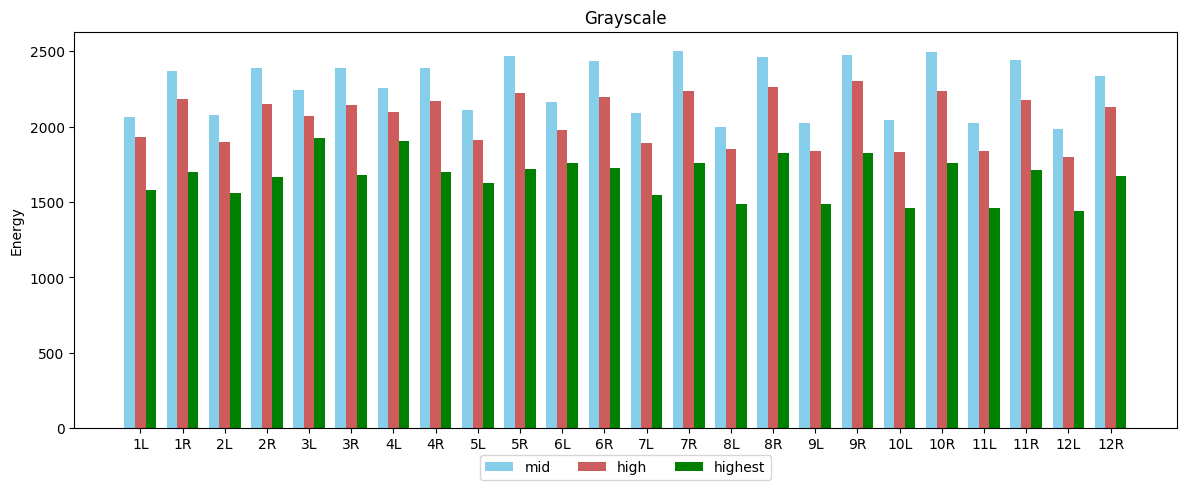
\includegraphics[scale=0.5]{images/appendix/stft/card/flattop_Grayscale.png}
        \caption{}
    \end{subfigure}\\
    \begin{subfigure}{\textwidth}
         \centering
          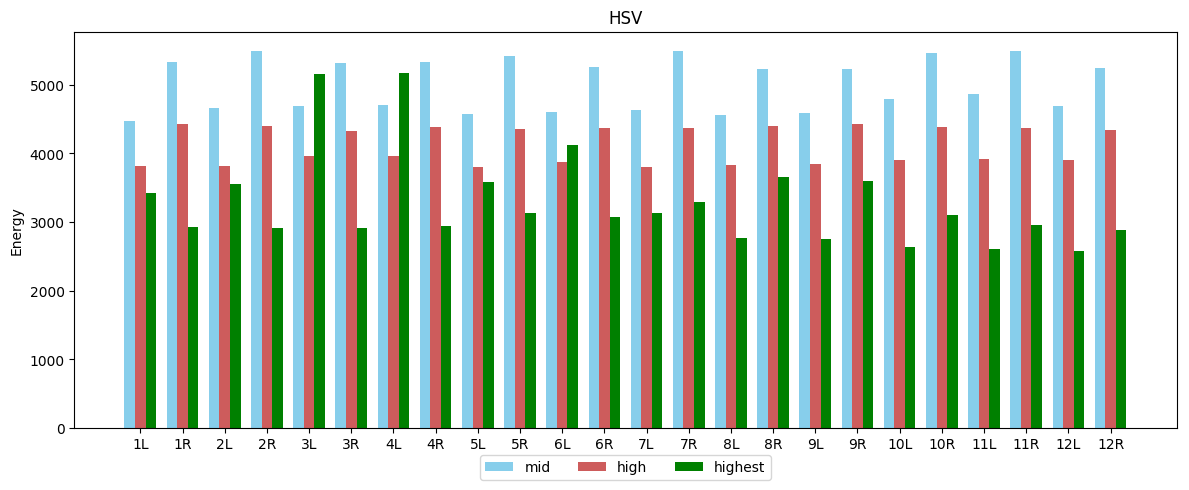
\includegraphics[scale=0.5]{images/appendix/stft/card/flattop_HSV.png}
          \caption{}
    \end{subfigure}
    \fautor
\end{figure}


\begin{figure}[H]
    \caption{Coin "v" STFT approach with Flattop window for Grayscale (a) and HSV (b) colourspaces.}
    \centering
    \begin{subfigure}{\textwidth}
        \centering
        \includegraphics[scale=0.5]{images/appendix/stft/coin_v/flattop_Grayscale.png}
        \caption{}
    \end{subfigure}\\
    \begin{subfigure}{\textwidth}
         \centering
          \includegraphics[scale=0.5]{images/appendix/stft/coin_v/flattop_HSV.png}
          \caption{}
    \end{subfigure}
    \fautor
\end{figure}

\section{Blackmanharris Window}

\begin{figure}[H]
    \caption{Airplane STFT approach with Blackmanharris window for Grayscale (a) and HSV (b) colourspaces.}
    \centering
    \begin{subfigure}{.5\textwidth}
        \centering
        \includegraphics[scale=0.41]{images/appendix/stft/airplane/blackmanharris_Grayscale.png}
        \caption{}
    \end{subfigure}%
    \begin{subfigure}{.5\textwidth}
         \centering
          \includegraphics[scale=0.41]{images/appendix/stft/airplane/blackmanharris_HSV.png}
          \caption{}
    \end{subfigure}
    \fautor
\end{figure}

\begin{figure}[H]
    \caption{Coin "o" STFT approach with Blackmanharris window for Grayscale (a) and HSV (b) colourspaces.}
    \centering
    \begin{subfigure}{\textwidth}
        \centering
        \includegraphics[scale=0.4]{images/appendix/stft/coin_o/flattop_Grayscale.png}
        \caption{}
    \end{subfigure}\\
    \begin{subfigure}{\textwidth}
         \centering
          \includegraphics[scale=0.4]{images/appendix/stft/coin_o/flattop_HSV.png}
          \caption{}
    \end{subfigure}
    \fautor
\end{figure}

\begin{figure}[H]
    \caption{Card STFT approach with Blackmanharris window for Grayscale (a) and HSV (b) colourspaces.}
    \centering
    \begin{subfigure}{\textwidth}
        \centering
        \includegraphics[scale=0.5]{images/appendix/stft/card/blackmanharris_Grayscale.png}
        \caption{}
    \end{subfigure}\\
    \begin{subfigure}{\textwidth}
         \centering
          \includegraphics[scale=0.5]{images/appendix/stft/card/blackmanharris_HSV.png}
          \caption{}
    \end{subfigure}
    \fautor
\end{figure}

\begin{figure}[H]
    \caption{Coin "v" STFT approach with Blackmanharris window for Grayscale (a) and HSV (b) colourspaces.}
    \centering
    \begin{subfigure}{\textwidth}
        \centering
        \includegraphics[scale=0.5]{images/appendix/stft/coin_v/blackmanharris_Grayscale.png}
        \caption{}
    \end{subfigure}\\
    \begin{subfigure}{\textwidth}
         \centering
          \includegraphics[scale=0.5]{images/appendix/stft/coin_v/blackmanharris_HSV.png}
          \caption{}
    \end{subfigure}
    \fautor
\end{figure}

\end{apendicesenv}
% ---


% ----------------------------------------------------------
% Anexos
% ----------------------------------------------------------

% ---
% Inicia os anexos
% ---
% \begin{anexosenv}

%     \chapter{Páginas interessantes na Internet} 
%     \label{chapter:paginas-interessantes}
%     \begin{description}
 \item[\url{http://www.tex-br.org}] Página em português com diversos tutoriais e referências interessantes sobre \LaTeX;
 \item[\url{http://en.wikibooks.org/wiki/LaTeX}] Livro em formato \textit{wiki} gratuito sobre \LaTeX;
 \item[\url{http://tobi.oetiker.ch/lshort/lshort.pdf}] Ótimo tutorial sobre \LaTeX (possui versão em português \url{http://alfarrabio.di.uminho.pt/~albie/lshort/ptlshort.pdf}, mas a versão em inglês é a mais atual);
 \item[\url{http://code.google.com/p/abntex2/}] Página do abnTeX2, grupo que desenvolve os pacotes e classes em \LaTeX para as normas da ABNT, nos quais a classe \textit{icmc} foi baseada;
\item[\url{http://www.more.ufsc.br}] Página do Mecanismo On-line para Referências  (MORE) desenvolvido pela UFSC;
\item[\url{http://detexify.kirelabs.org/classify.html}] Página para recuperar o código de símbolos em \LaTeX a partir do desenho fornecido pelo usuário.
 \end{description}

% \end{anexosenv}
% ---

\end{document}